%!TEX root=../../../main.tex
Selve jordfugtsensoren skal måle fugten i jorden således at systemet kan vide hvornår et givent medie skal have vand. 

Da det ønskes at sensoren skal kommunikere over I2C på en selvdesignet protokol, ønskes det samtidig at levere en speciallavet jordfugtsensor til systemet. Dette kræver at der designes én fra bunden.\newline 

\subsection{Kapacitiv måling}
Den første ide til at måle jordfugten gik ud på at måle den kapacitivt. Efter nogle hurtige søgninger på Google blev der hurtigt fundet frem til følgende dokument \footnote{\citet{transem:humiditysensor}}
I pdf filen beskriver to japanske studerende hvordan de med en kapasitet er i stand til at måle den relative luftfugtig. Dette virker ved at når luftfugtigheden ændre sig kan man via to elektrisk ledende plader måle forskellen i luften ved at koble dem som en pladekondensator med luften som dielektrikum. 
$\epsilon$r ændre sig således med luftfugtigheden. Tanken var nu at det samme måtte gøre sig gældende for jorden og komponenten i figur \ref{photo:Kapsitiv_foeler} blev lavet:

\begin{figure}[H]
	\centering 
	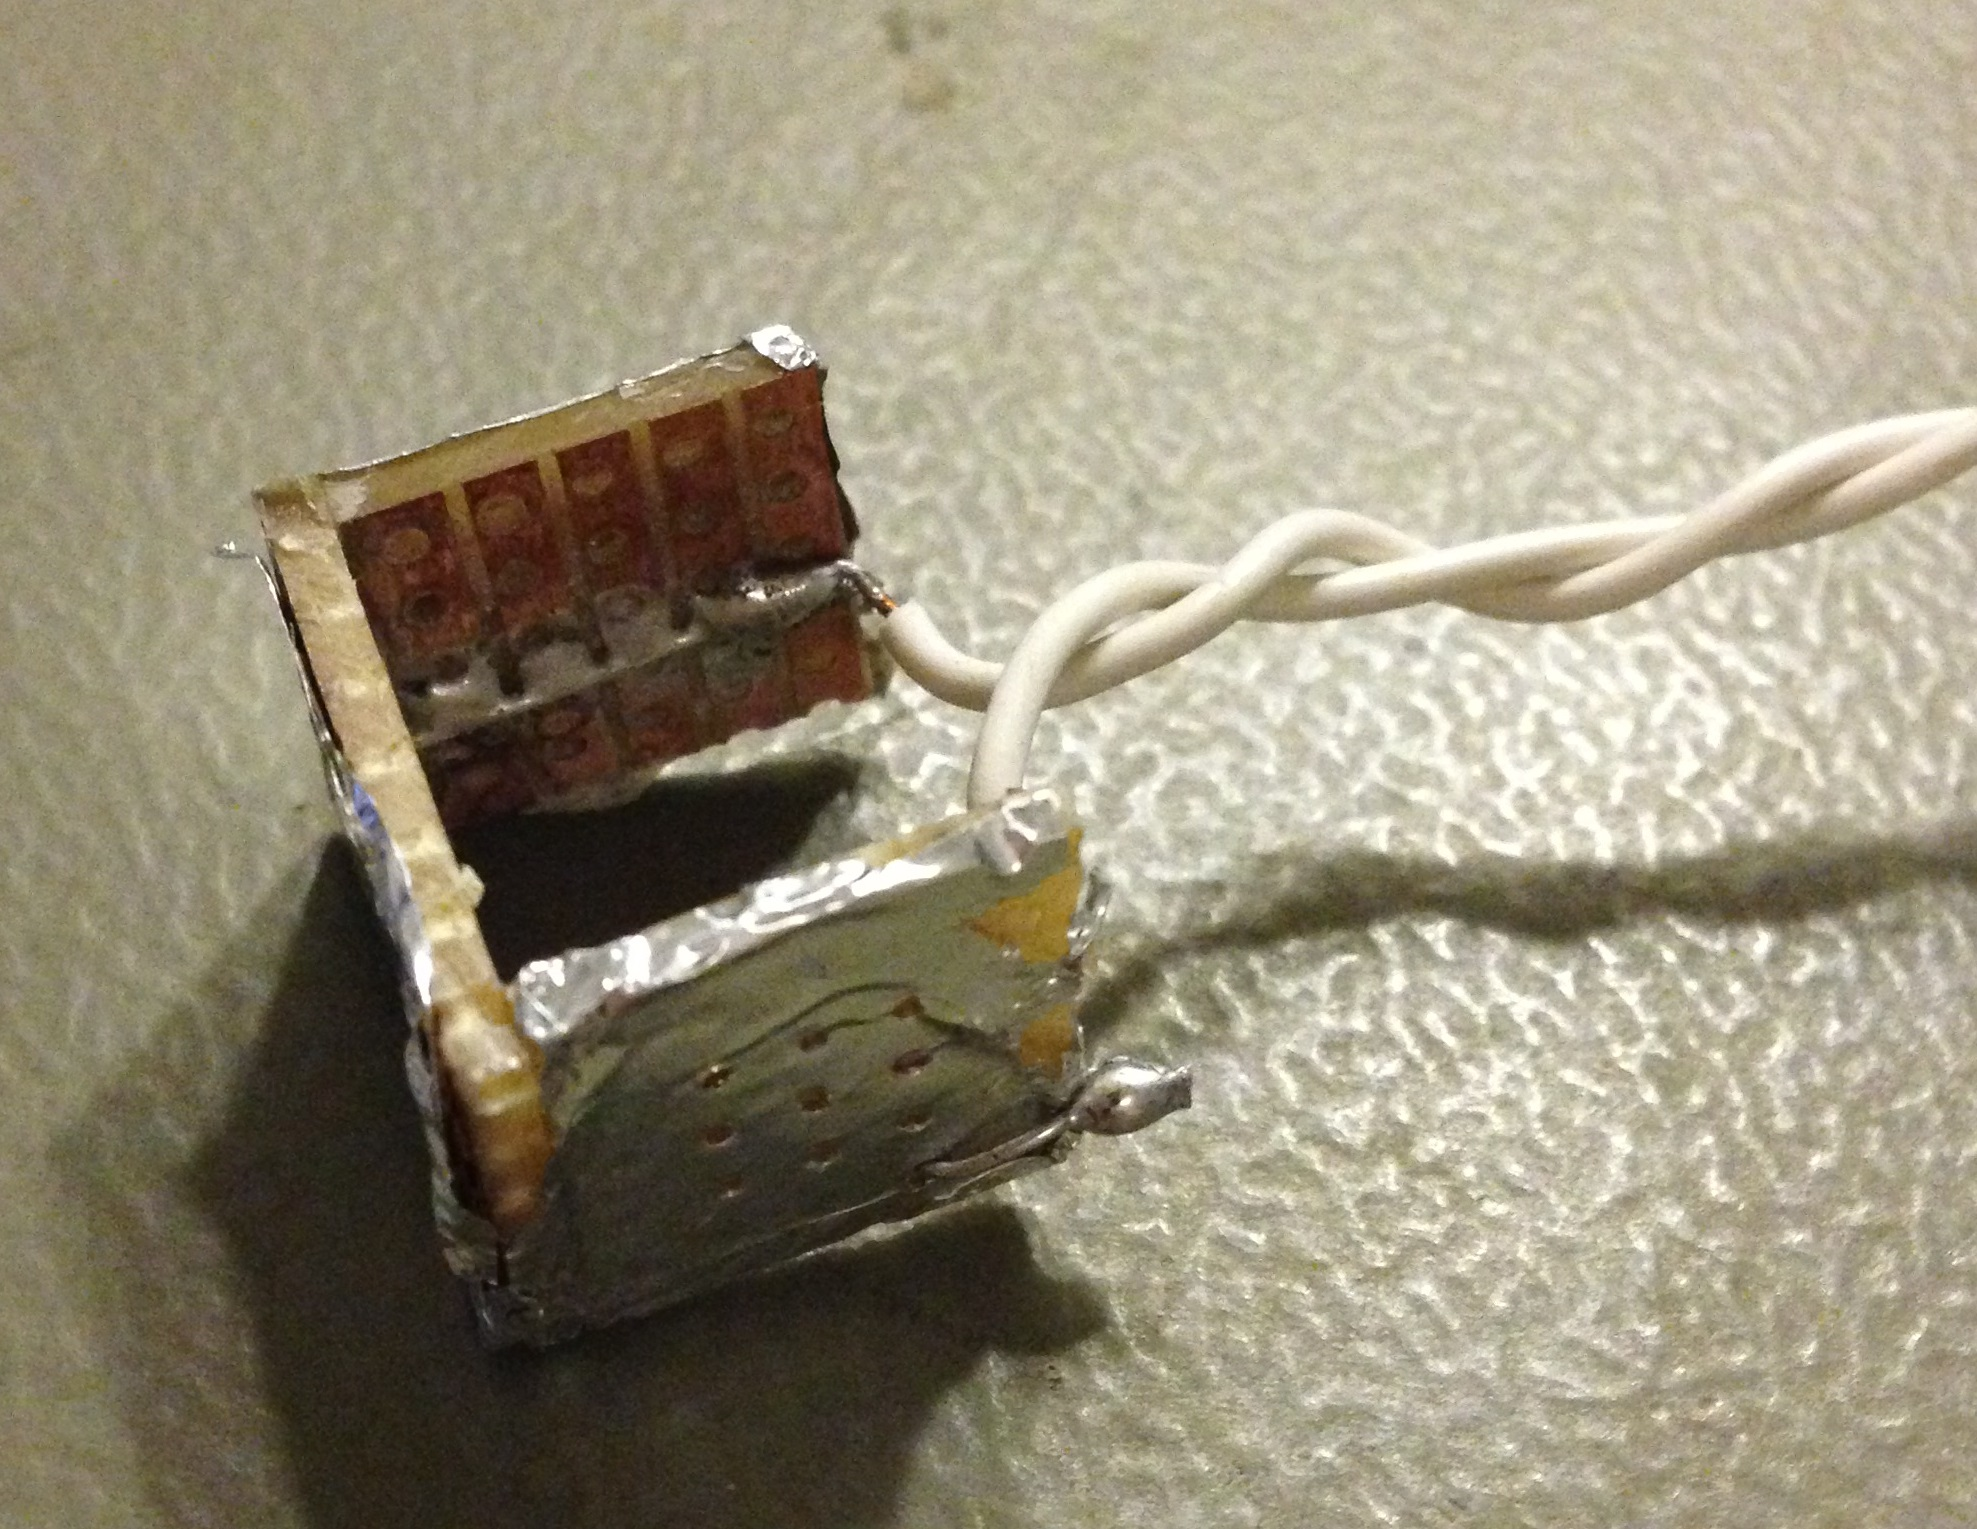
\includegraphics[scale=0.1]{HardwareArkitektur/Sensore/Jordfugt_billeder/Kapacitiv_foler.JPG}
	\caption{Opbygning af den kapacitive f$\text{ø}$ler}
	\label{photo:Kapsitiv_foeler}
\end{figure}

Til den hjemmebyggede pladekondensator blev der også opbygget en oscillator som varierede sin udgangsfrekvens afhængig af kondensatorens kapacitet. Dette kredsløb blev bygget med en LM555. Da pladekondensatoren var en kopi fra det før omtalte pdf dokument kom det ikke som en overraskelse at oscillatoren ændrede sin frekvens med næsten 50\% når pladekondensatoren blev holdt over dampen fra en kop kogende vand. Hvad der dog ikke var taget højde for var kapaciteten i tilledningerne, som ændrede sig hver gang pladekondensatoren blev flyttet. Det viste sig også at når pladekondensatoren blev trykket ned i jord stoppede oscillatoren med at oscillere. Det var hellere ikke muligt at måle kapaciteten med et LCR-meter og ideen blev derfor opgivet.\newline

\subsection{Resistiv måling}
Næste step var at finde en ny metode til at måle fugtigheden i jorden og denne opstod ved besøg på denne side \footnote{\citet{gardenbot:soilmoisture}} På siden bliver det beskrevet hvordan fugtigheden i jorden kan måles rent resistivt. Desværre bliver der ikke givet nogle værdier på jordens ledeevne i forhold til fugtigheden og var derfor op til én selv at finde den. Ved en større søgning blev der fundet frem til oversigten i figur \ref{photo:Ledeevne_grundstoffer} Kilde\footnote{\citet{zonge:soilpermability}}

\begin{figure}[H]
	\centering 
	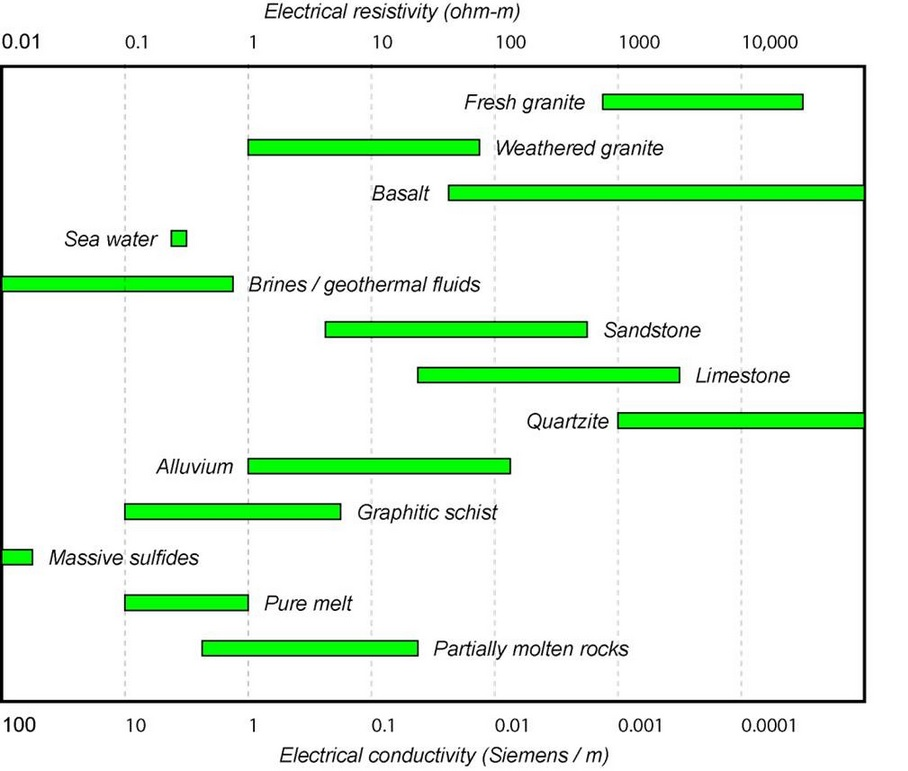
\includegraphics[scale=0.5]{HardwareArkitektur/Sensore/Jordfugt_billeder/soil_conductivity_types.JPG}
	\caption{Oversigt over ledeevnen for nogle forskelige grudstoffer.}
	\label{photo:Ledeevne_grundstoffer}
\end{figure}

Det ses her at f.eks. Sandsten varierer fra en ledeevne på 0.5 til 0.003 Siemens/m. Dette er et meget stort spektrum og det vil derfor være umuligt at sige noget om ledeevnen i jorden uden først at have målt den. For at kunne gøre dette krævede det at der blev lavet et jordspyd der kunne bruges til at lave målingen med. I figur \ref{photo:Ledeevne_grundstoffer} ses jordspyddet sænket ned i vand fra vandhanen, for at måle vandets ledeevne. Da jordspyddet er delvist isoleret med krympeflex er det et fast areal på begge spyd der er i kontakt med vand, og derfor vil det være muligt at beregne ledeevnen for vandet.

\begin{figure}[H]
	\centering 
	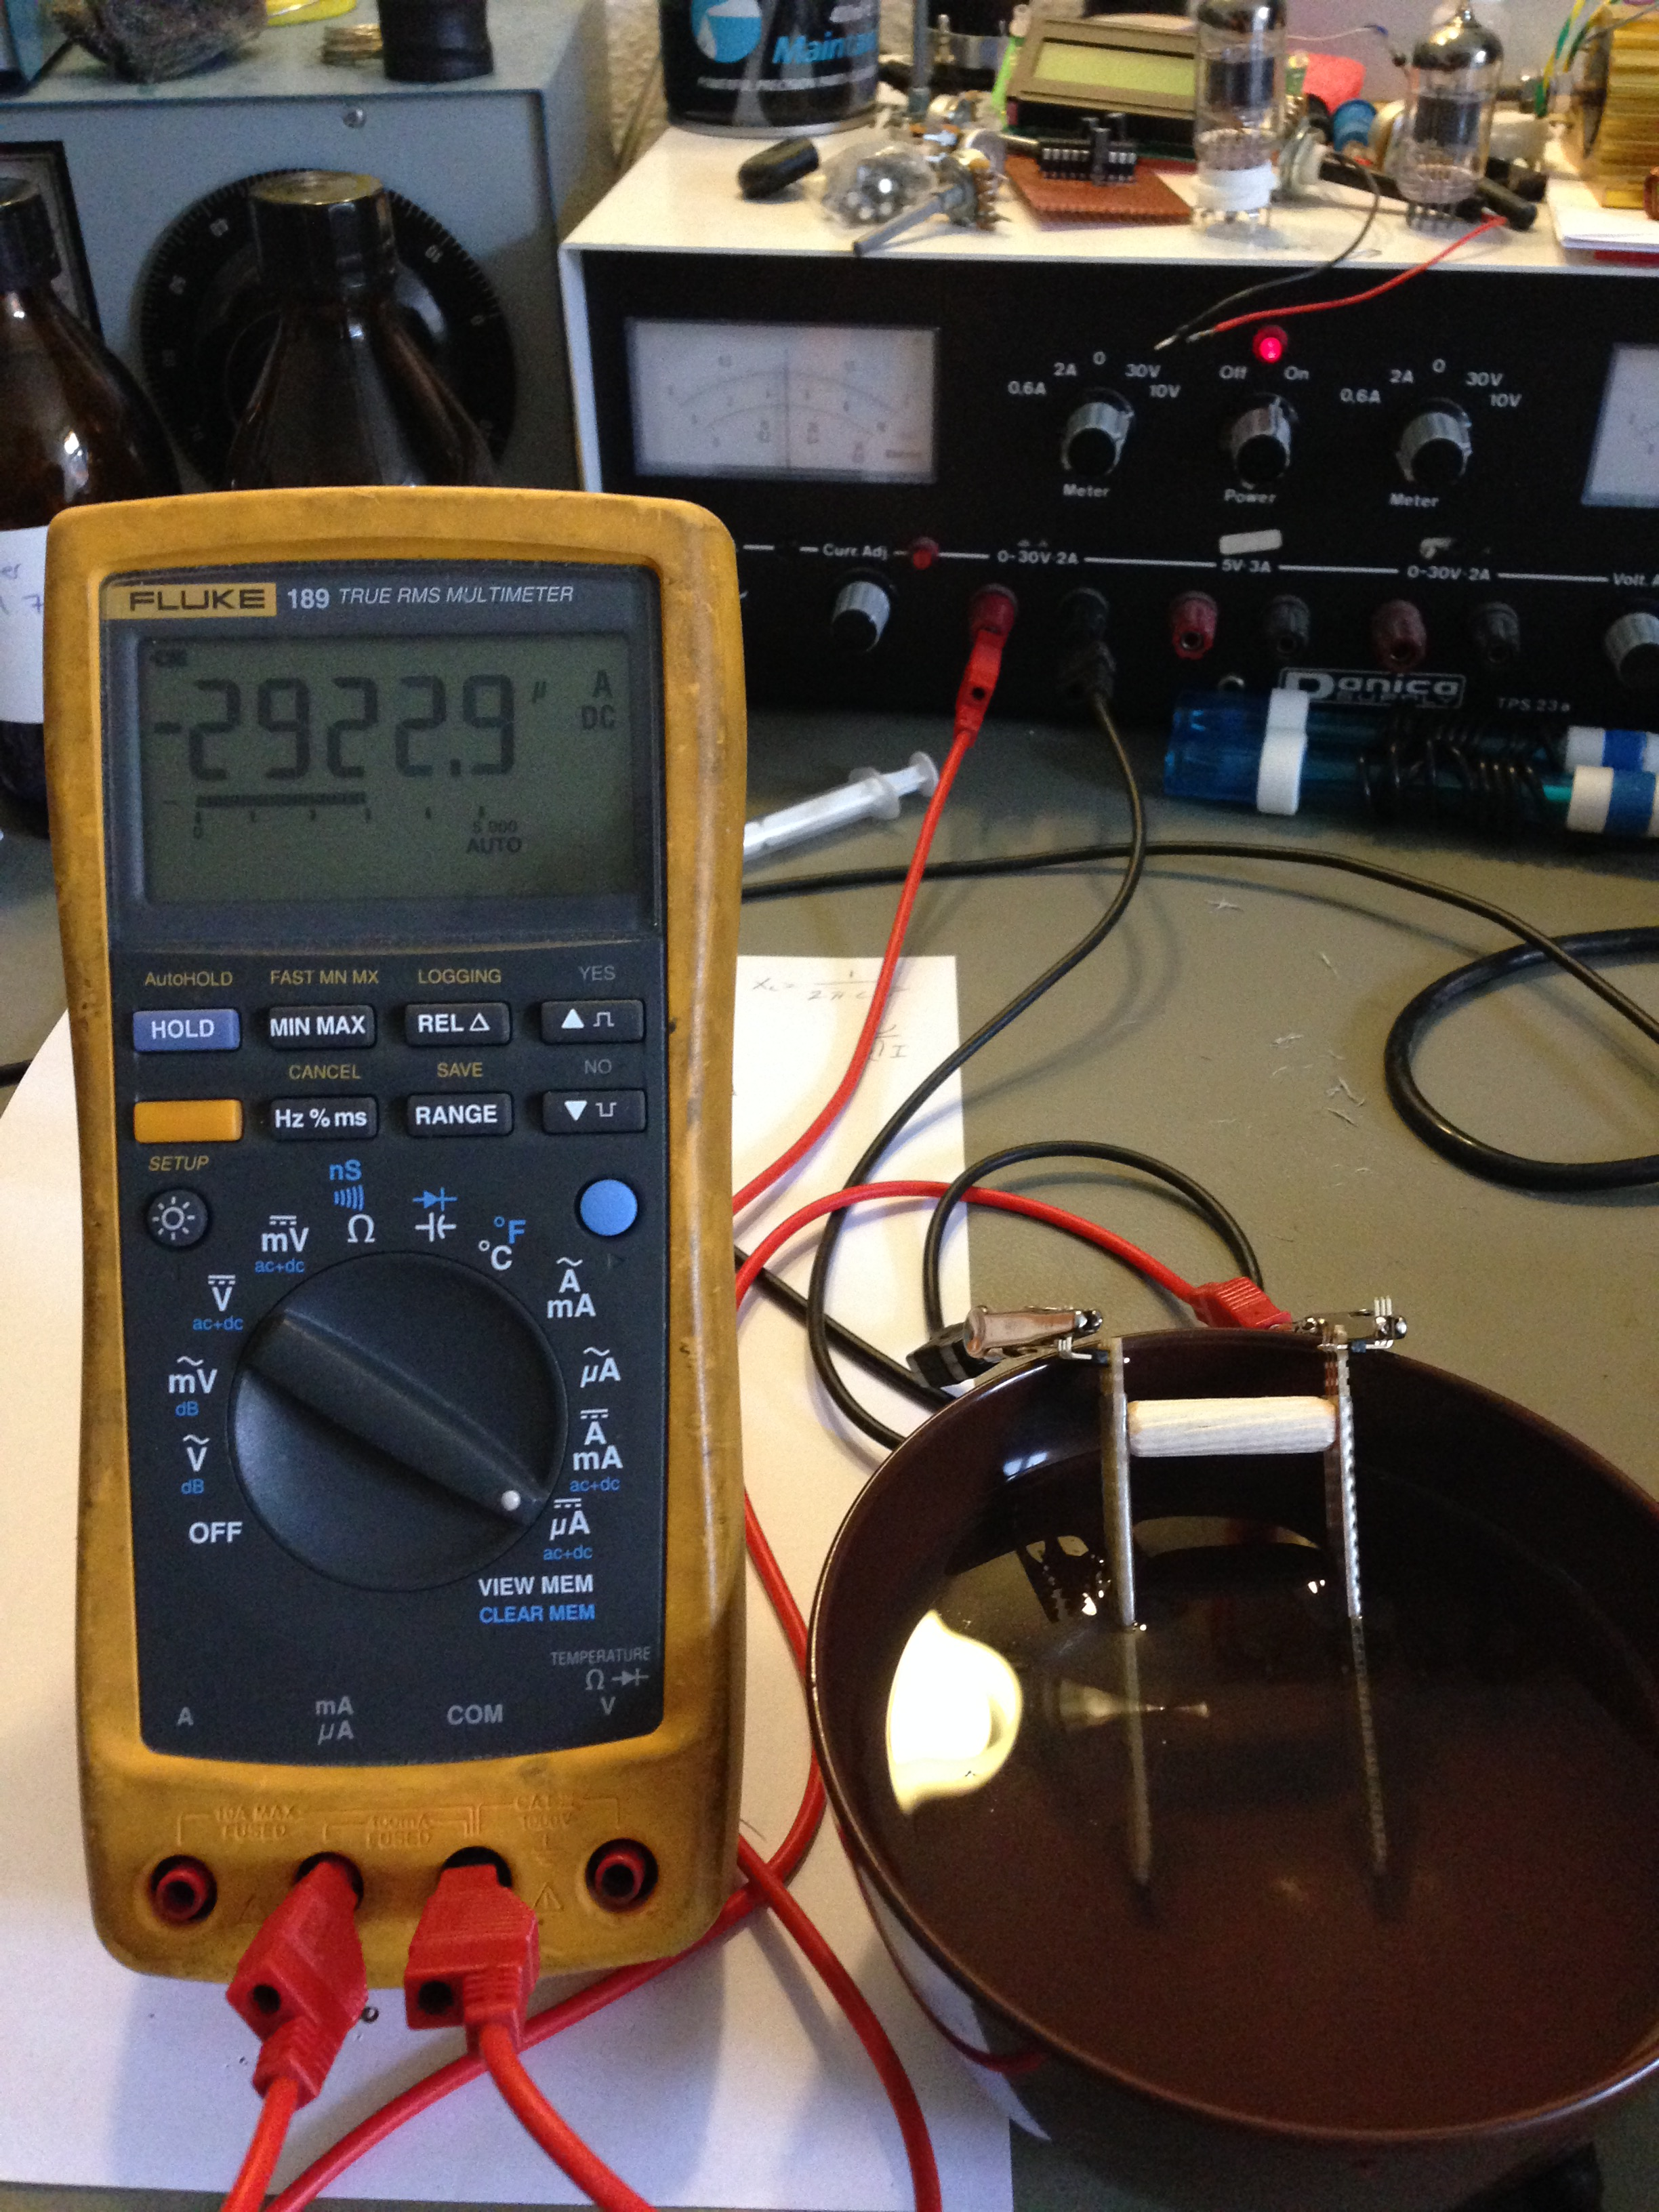
\includegraphics[scale=0.07]{HardwareArkitektur/Sensore/Jordfugt_billeder/Jordspyd_i_vand.JPG}
	\caption{Multimeteret måler strømmen igennem jordspyddet ved en spænding på 5V (2.92mA}
	\label{photo:Jordspyd_vand}
\end{figure}  

\begin{figure}[H]
	\centering 
	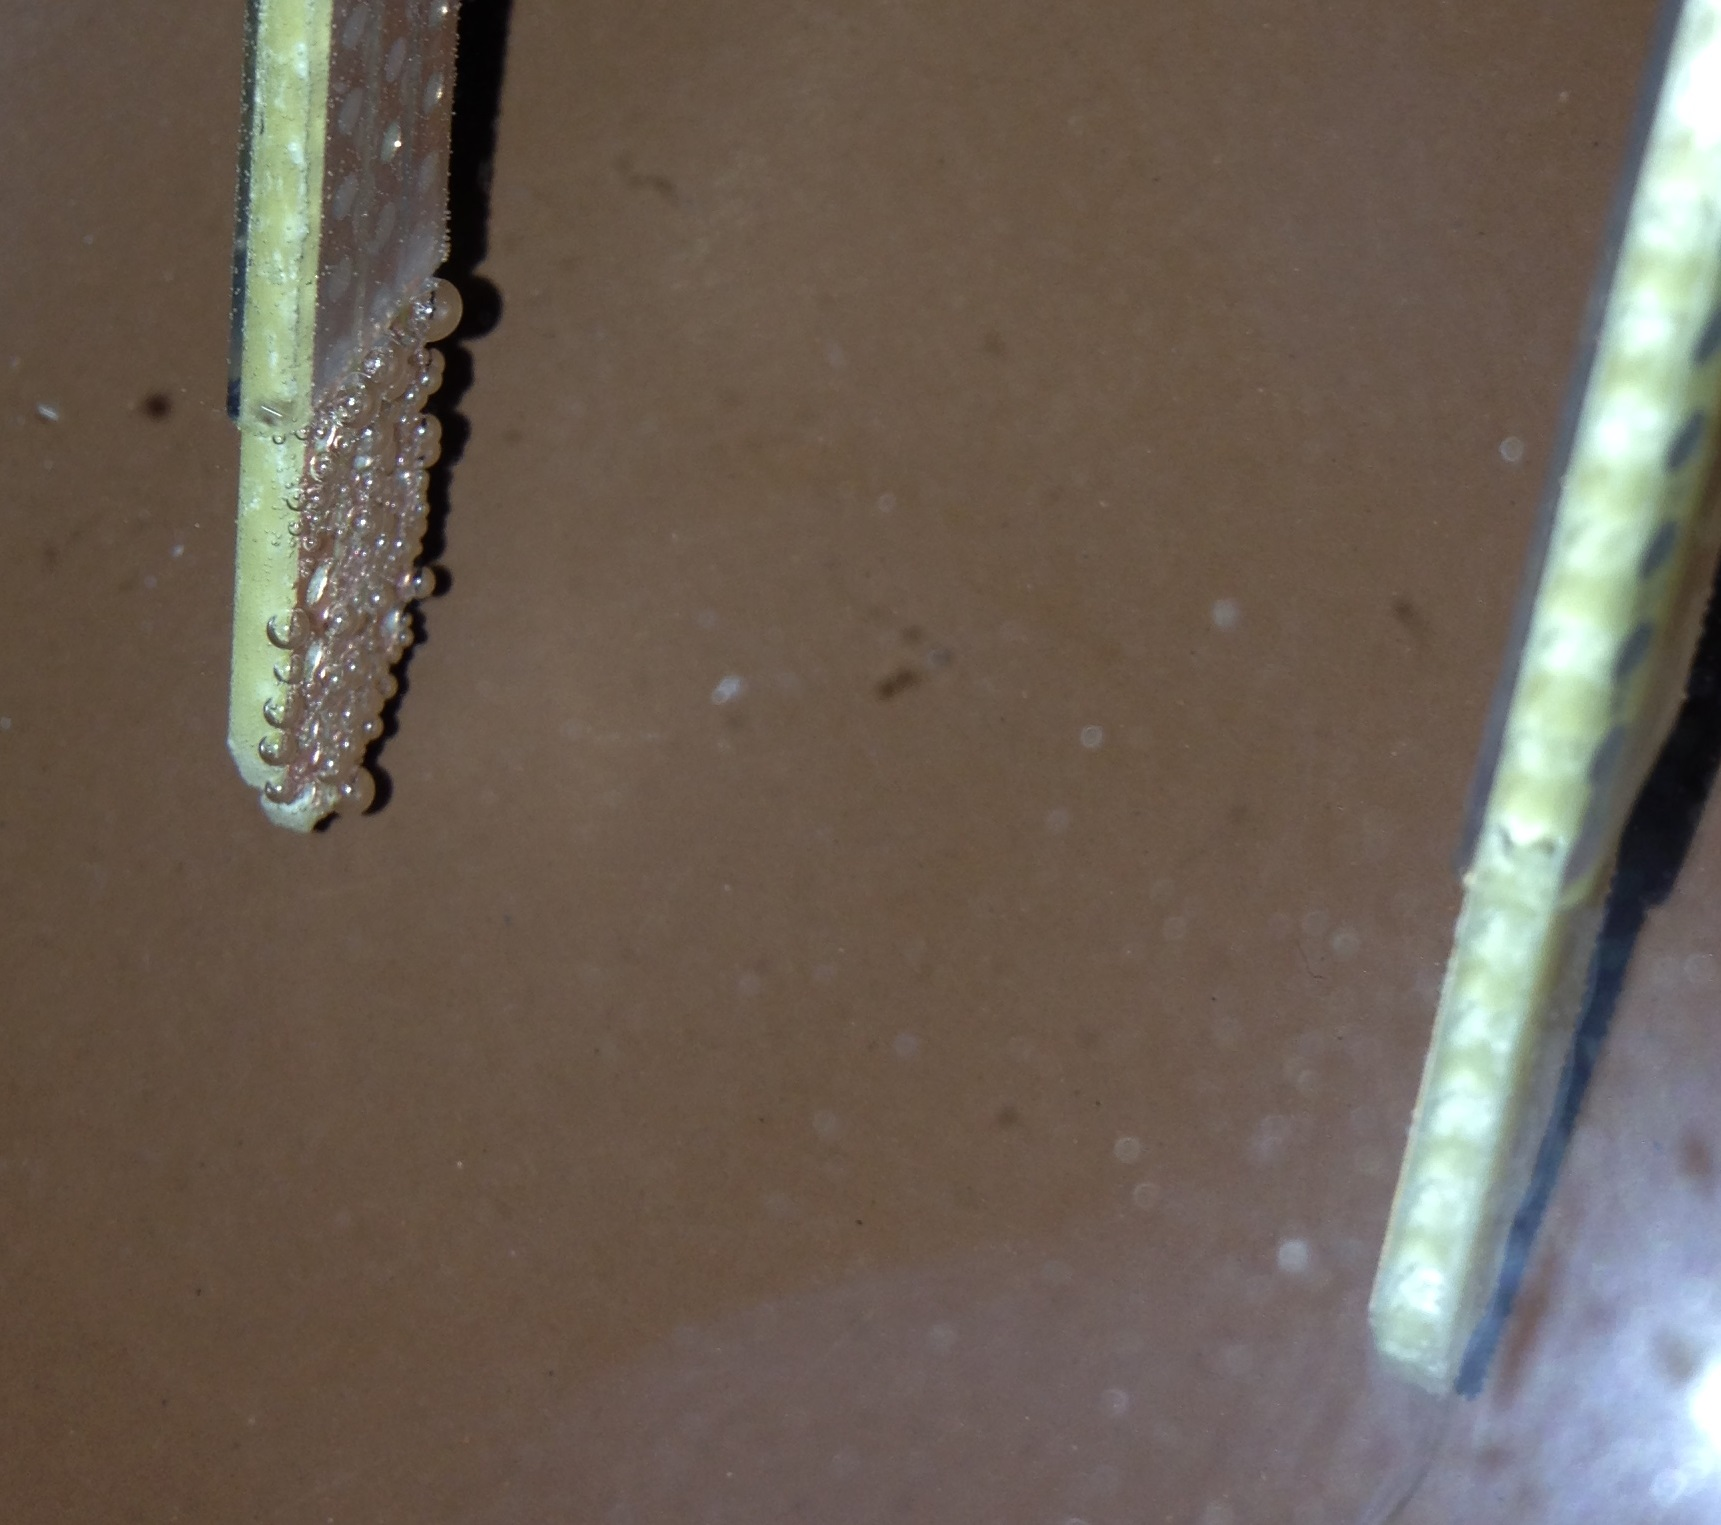
\includegraphics[scale=0.1]{HardwareArkitektur/Sensore/Jordfugt_billeder/Elektrolyse.JPG}
	\caption{Elektrolyse ved 5V}
	\label{photo:Elektrolyse}
\end{figure}  

På figur \ref{photo:Elektrolyse} ses at der desværre også forekommer elektrolyse ved denne målemetode. Der ses at katoden tiltrækker hydrogen-atomer som sætter sig som luftbobler på kobberet. Ved en spænding på 30V var elektrolysen så kraftigt at kobberlaget på anoden ville være væk efter få minutter. Derfor konstanters det også at ved implementering af denne type måling må der kun gå strøm i jordspyddet i det øjeblik målingen bliver foretaget, for at undgå unødvendig slid.\newline

Den mest interessante opdagelse blev gjort ved måling i jorden. Her var teorien at ledeevnen ville stige lineært med fugtigheden. Denne antagelse viste sig at være forkert, og ved plotning af målepunkterne i koordinatsystem, lignede det trendlinjen i stedet et stigende 4. polynomium. Forinden havde det været et stort problem at finde ud af hvilken måleskala der skulle benyttes til måling af fugtigheden, da der findes mange definitioner heraf. Der blev fundet frem til at fugtigheden i tørvægt var den mest brugbare for geoteknikere og derfor blev denne skala der blev valgt. Skalaen angiver, at hvis der er 100 gram ovntørret jord og 40 gram vand indeholder jorden 40\% fugtighed. I formlen står m for masse.
$$ \mu = \frac{m_{wet}-m_{dry} }{m_{dry}}$$ \newline

På figur \ref{photo:Opvejning} og \ref{photo:Maetningspunkt} ses hvordan målingerne af jordfugtigheden blev foretaget. 

\begin{figure}[H]
	\centering 
	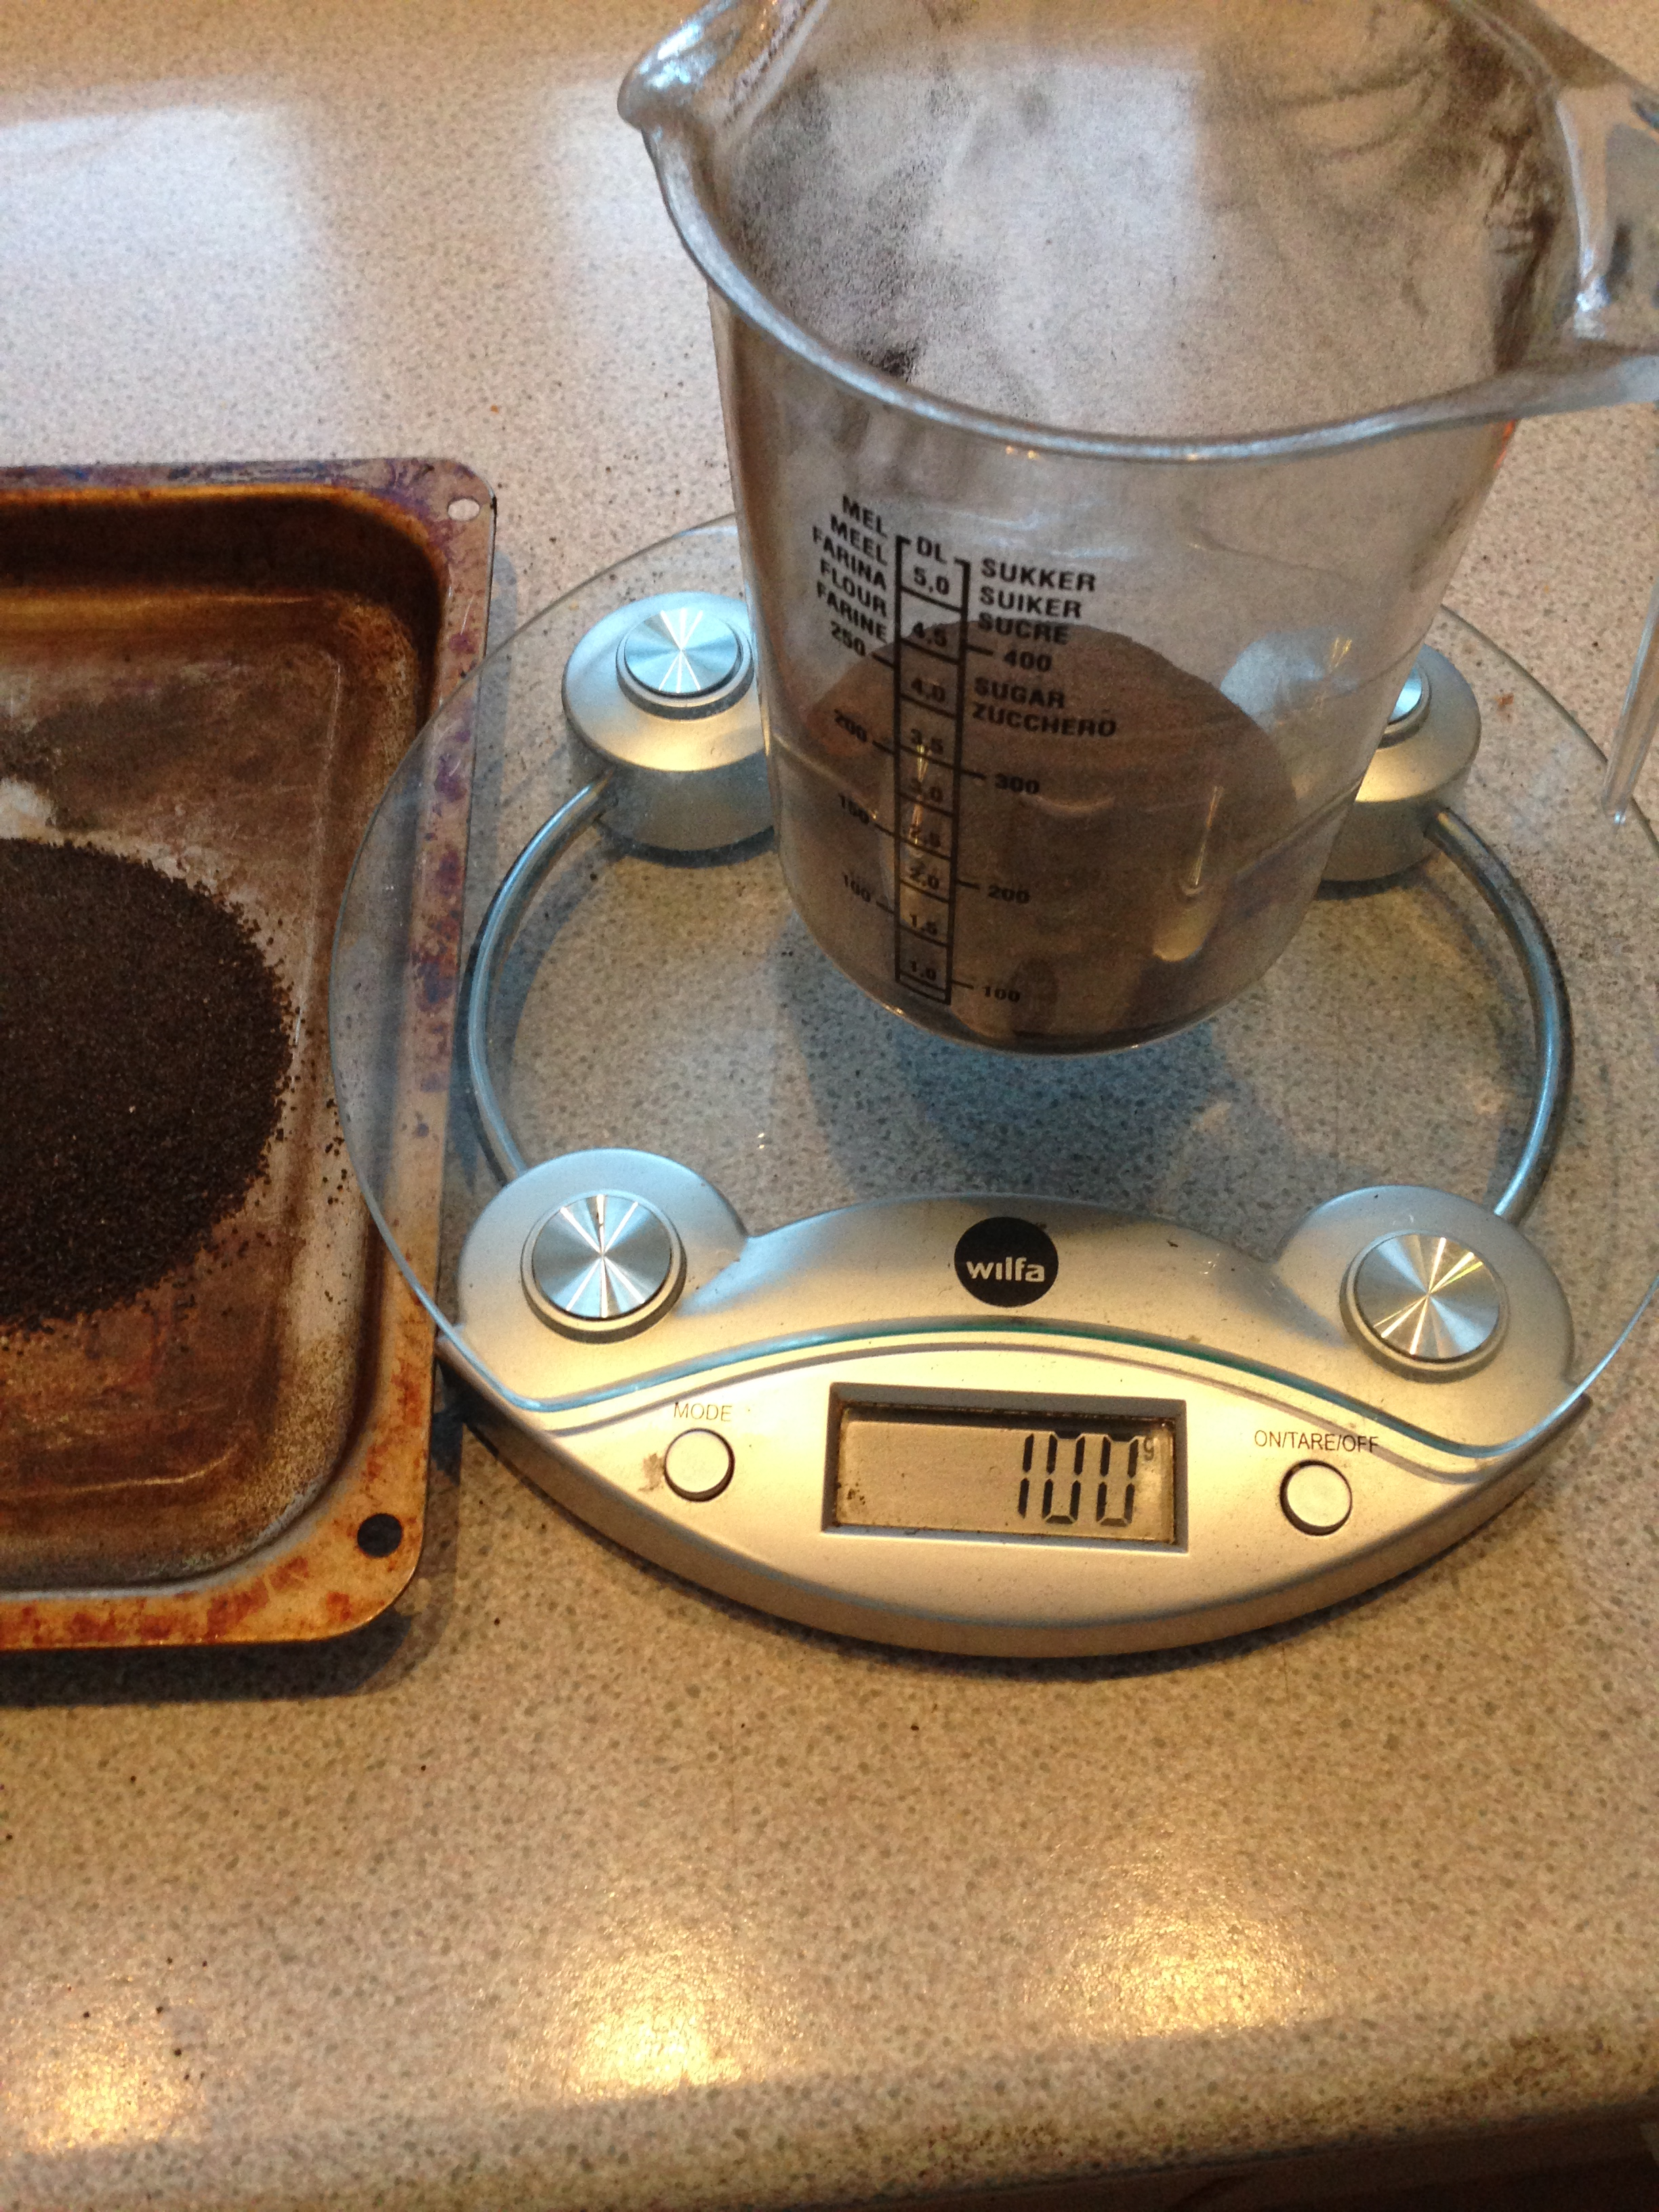
\includegraphics[scale=0.08]{HardwareArkitektur/Sensore/Jordfugt_billeder/Opvejning.JPG}
	\caption{Vejning af 100 gram af ovntørret jord. Vægten er nulstillet med tomt målebægre}
	\label{photo:Opvejning}
\end{figure}  
 
\begin{figure}[H]
	\centering 
	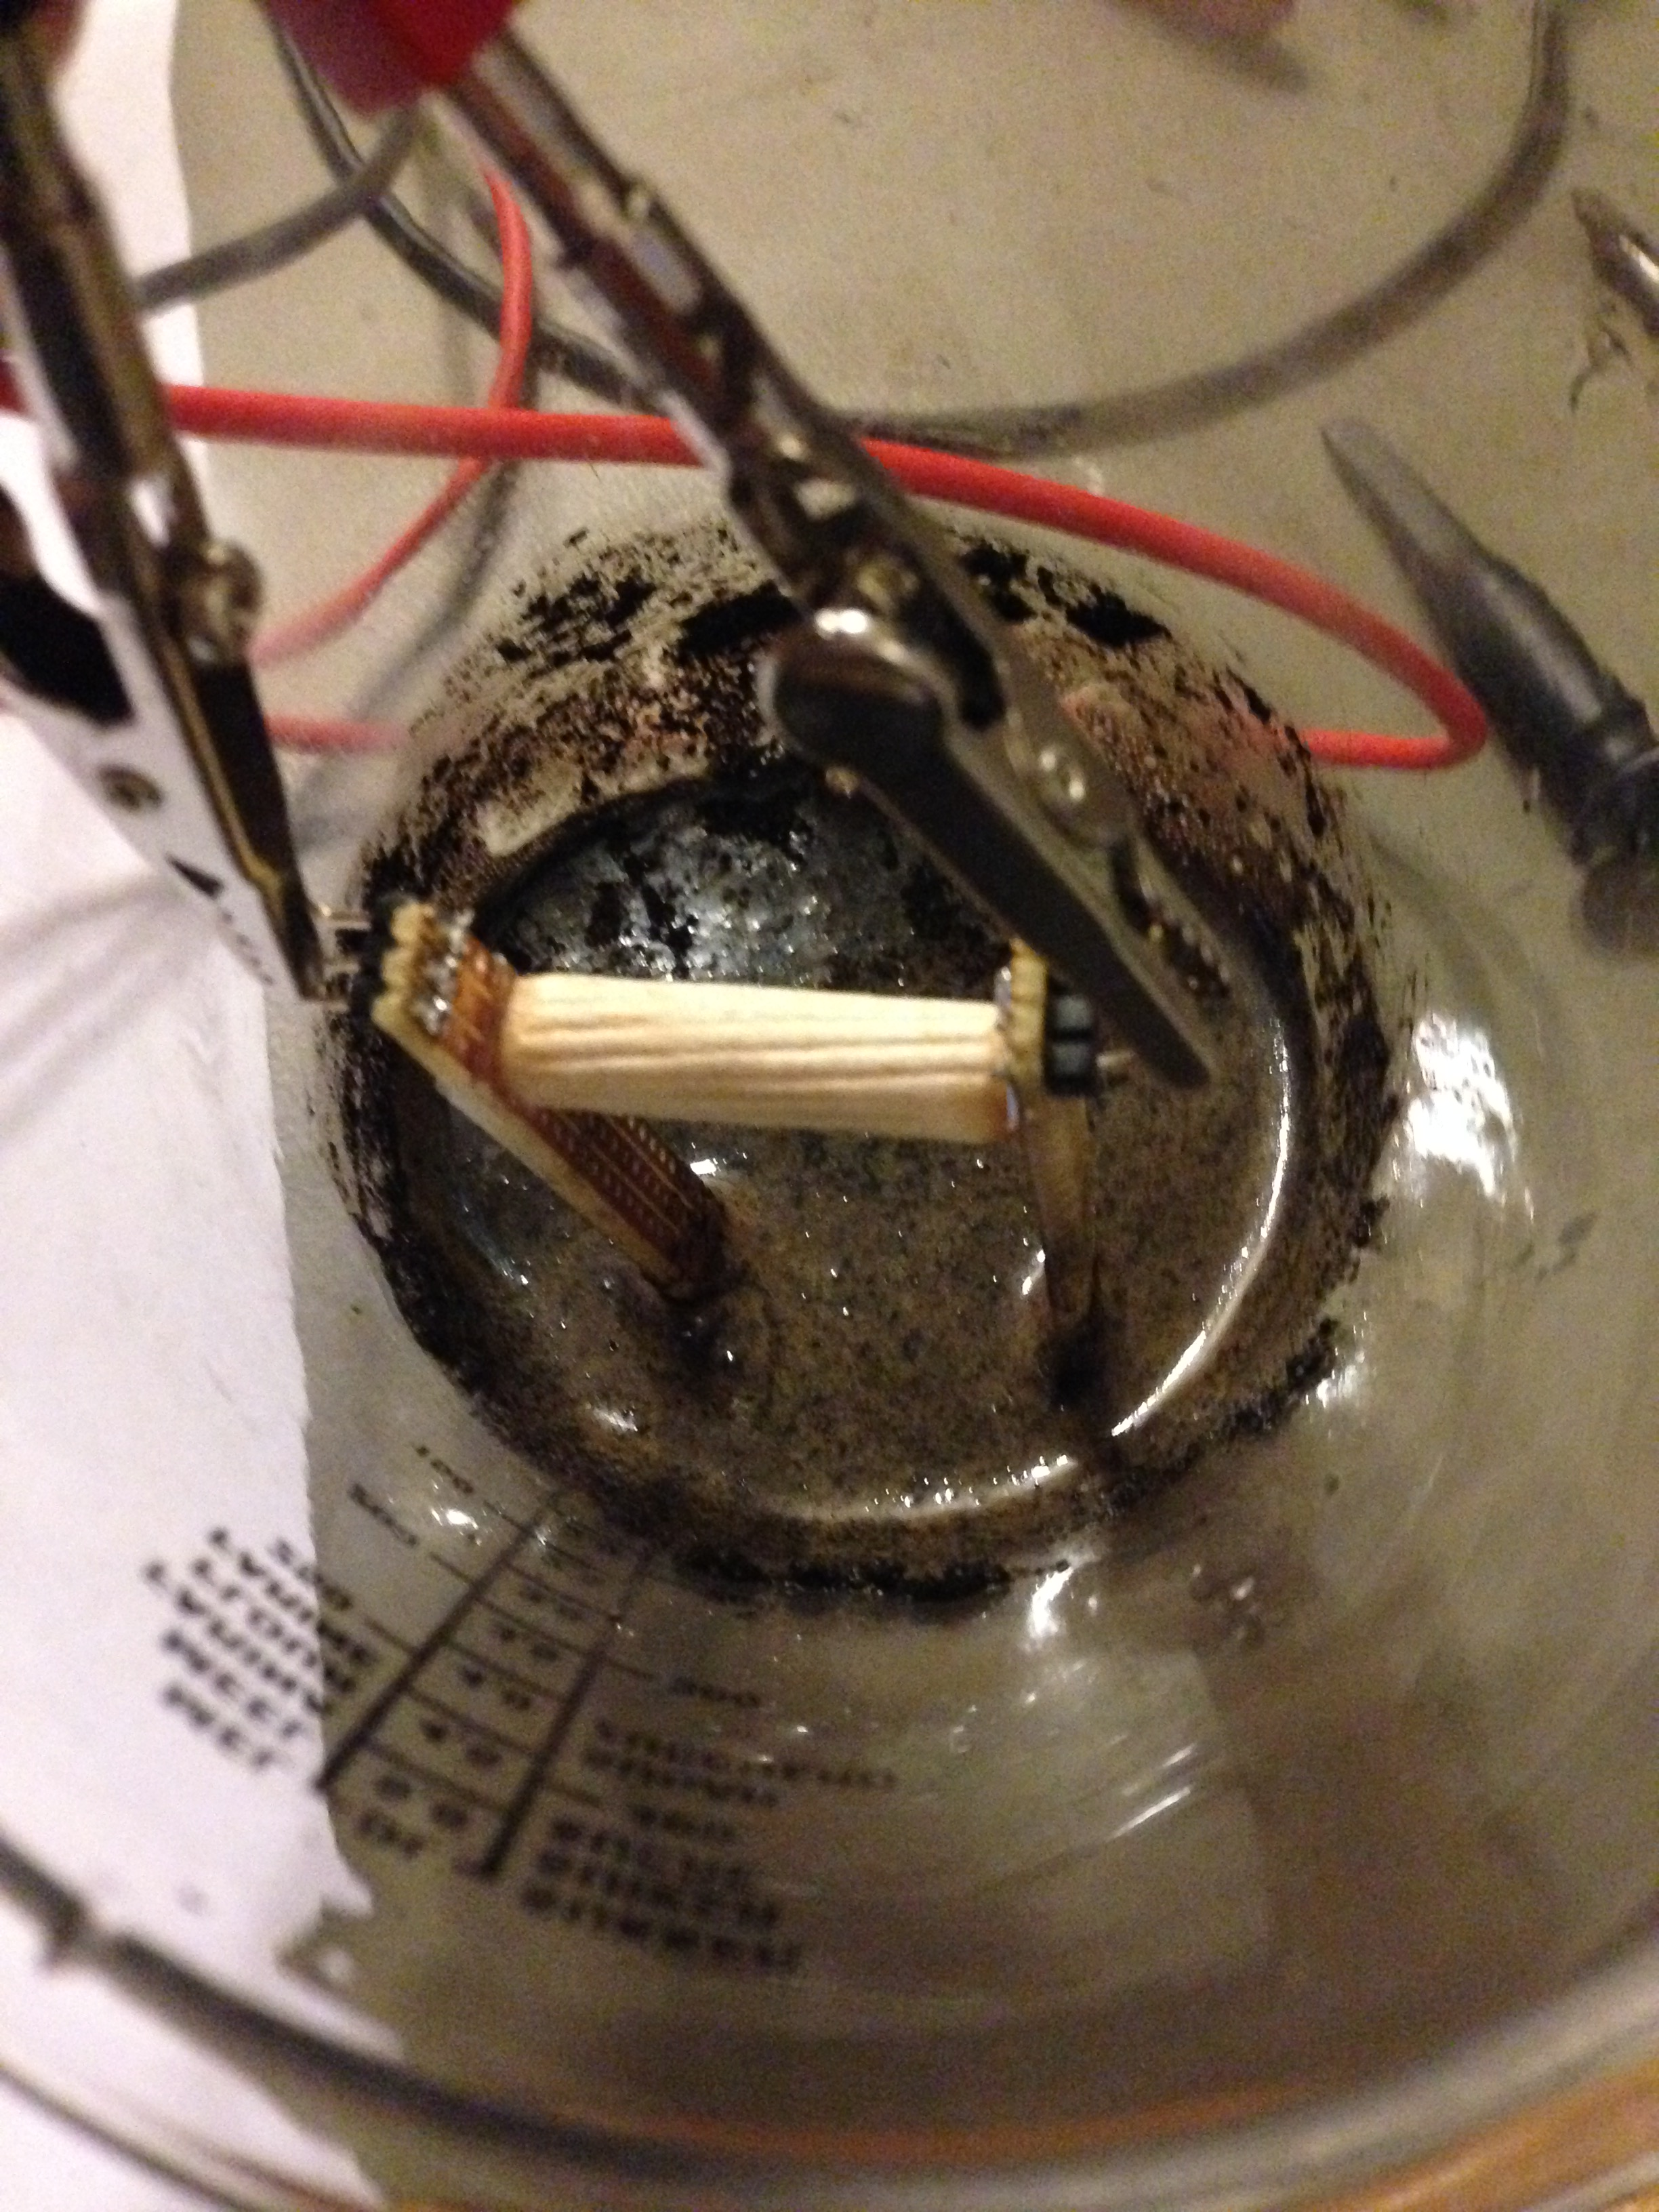
\includegraphics[scale=0.08]{HardwareArkitektur/Sensore/Jordfugt_billeder/Maetningspunktet.JPG}
	\caption{Her ses blandingsforholdet hvor strømmen i jordspyddet igen er faldende}
	\label{photo:Maetningspunkt}
\end{figure}  

På figur \ref{photo:Maetningspunkt} blev der foretaget 7 målinger ved varierende fugtighed. Ved en fugtighed på 25.6\% begyndte strømmen i jordspyddet at falde igen. Dette bliver et problem i det samlede system da systemet ikke kan vide om den måler i en overvandet plante. På fig.\ref{photo:Graph_jordfugtighed} ses regression af målepunkterne. 

\begin{figure}[H]
	\centering 
	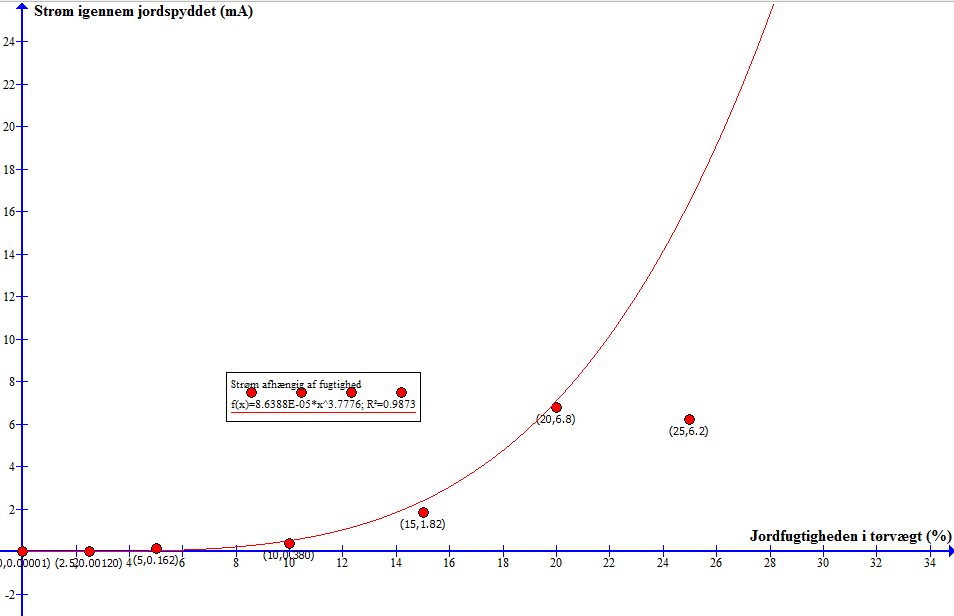
\includegraphics[scale=0.6]{HardwareArkitektur/Sensore/Jordfugt_billeder/Graph_jordfugtighed.PNG}
	\caption{Målinger indtegnet i Graph. Den yderste måling til højre (25,6.2) er det før omtalte "knæk punkt" hvor vi ikke længere ved om vi måler rigtigt. punktet er ikke medtaget i regressionen.}
	\label{photo:Graph_jordfugtighed}
\end{figure}  

På figur \ref{photo:Graph_jordfugtighed} aflæses regressionen af grafen til:
$$f(x) = 8.64*10^{-5}x^{3.77} $$
Funktionen er udtryk for strømmen i jordspyddet ved en given fugtighed. Dette kan med fordel omskrives til modstand ved brug af ohms lov. Den påtrykte spænding fra spændingsgeneratoren er 5V
$$f(x) = \frac{5V}{{8.6388*10^{-5}*x^{3.78}*10^{-3}A}}$$
Denne funktion kan bruges i en MCU med en analog til digital konverter, således strømmen kan omregnes til jordfugtighed i procent. På figur \ref{photo:jordspyd_modstand} ses plot af funktionen. 

\begin{figure}[H]
	\centering 
	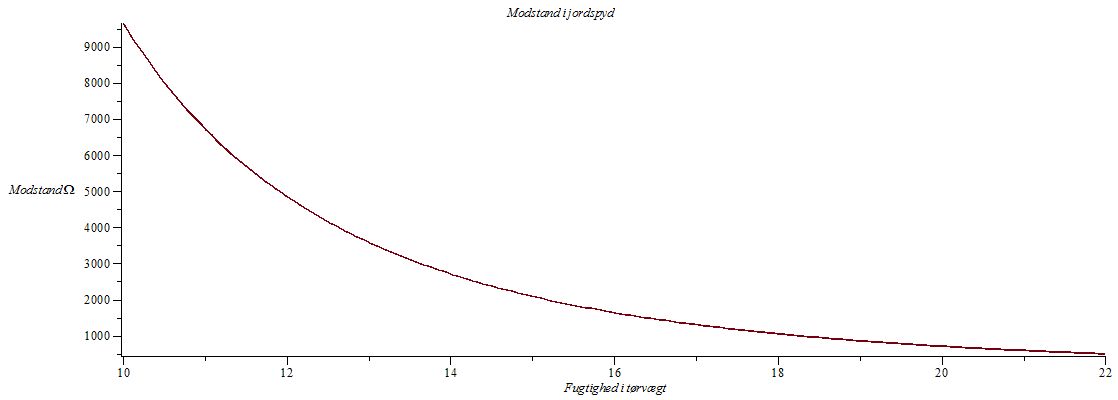
\includegraphics[scale=0.4]{HardwareArkitektur/Sensore/Jordfugt_billeder/jordspyd_modstand.PNG}
	\caption{Plot over modstand i jordspyddet ved en given fugtighed. Grafen er et udsnit fra 10\% til 22\% for at gøre den mere overskuelig}
	\label{photo:jordspyd_modstand}
\end{figure}  

\subsection{Test og opbygning}
Næste punkt er at finde en metode til at måle modstanden i spyddet. Dette kan gøres ved at koble jordspyddet som spændingsdeler med en MOSFET-transistor til at lede strømmen når der måles. På figur \ref{photo:jordspyd_diagram} ses diagrammet over forklaringen. 
 
\begin{figure}[H]
	\centering 
	\includegraphics[scale=0.8]{HardwareArkitektur/Sensore/Jordfugt_billeder/jordspyd.JPG}
	\caption{Diagram over jordspyddet}
	\label{photo:jordspyd_diagram}
\end{figure} 

Følgende funktion opstilles for kredsløbet:
$$Rspyd=-{\frac {{Vout}\,{R1}}{{Vout}-{Vcc}}}$$
Ved at isolere x i funktionen på fig.\ref{photo:jordspyd_modstand} fås et udtryk for fugtigheden hvis modstanden er kendt. 
$$fugt=\frac{113.47}{Rspyd^{0.26472}}$$
Disse to formler bliver brugt i PSoC-Creator til at programmere CY8C4245AXI-483 chippen med en differentielkoblet analog til digital konverter. På fig.\ref{photo:ADC} ses topdesignet i PSoC-Creator.    

\begin{figure}[H]
	\centering 
	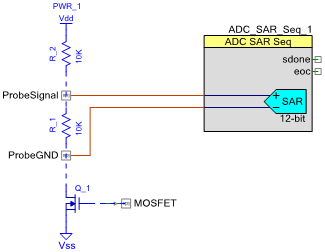
\includegraphics[scale=0.8]{HardwareArkitektur/Sensore/Jordfugt_billeder/SAR_converter.png}
	\caption{Topdesign i PSoC creator}
	\label{photo:ADC}
\end{figure} 

I PSoC-Creator oprettes en funktion der udlæser værdien fra ADC'en og omregner den til fugtighed. Kredsløbet opbygges på fumlebræt, med et 4.7k potientometer, samt en 100ohms modstand koblet serielt. På fig. \ref{photo:debug100} ses debugging af første iteration af funktionen.

\begin{figure}[H]
	\centering 
	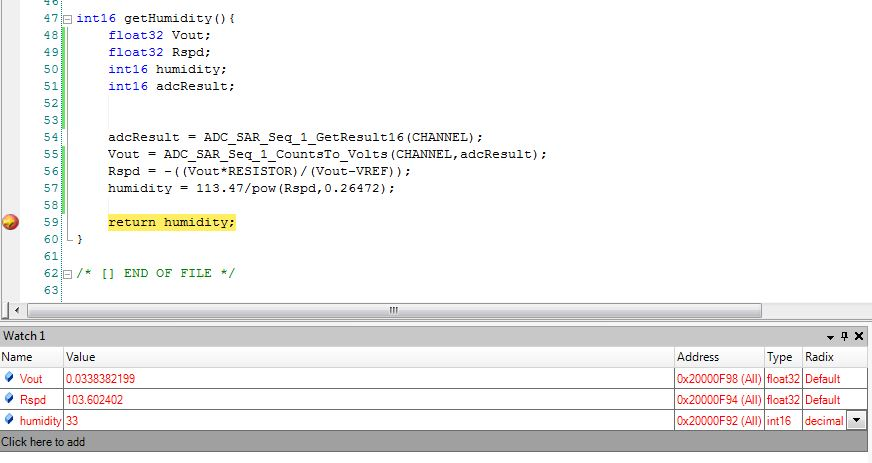
\includegraphics[scale=0.8]{HardwareArkitektur/Sensore/Jordfugt_billeder/debug100ohm.jpg}
	\caption{Debugging i PSoC creator ved Rspyd=100$\Omega$}
	\label{photo:debug100}
\end{figure} 

Aflæses 100$\Omega$ på fig.\ref{photo:jordspyd_modstand} ses det at, en fugtighed på 33, stemmer fint overens med det forventede og funktion antages efter flere lignende resultater at virke efter hensigten. Efterfølgende er funktionen lavet om således den også kommunikerer med sensor Ø'en. Den færdige kode findes i bilagene under SoftwareArkitektur.\newline

Efterfølgende oprettes et kredsløbsdiagram i DesignSpark, og i samme program udarbejdes printlayout. Dette layout ses på fig.\ref{photo:Print_2}.

\begin{figure}[H]
	\centering 
	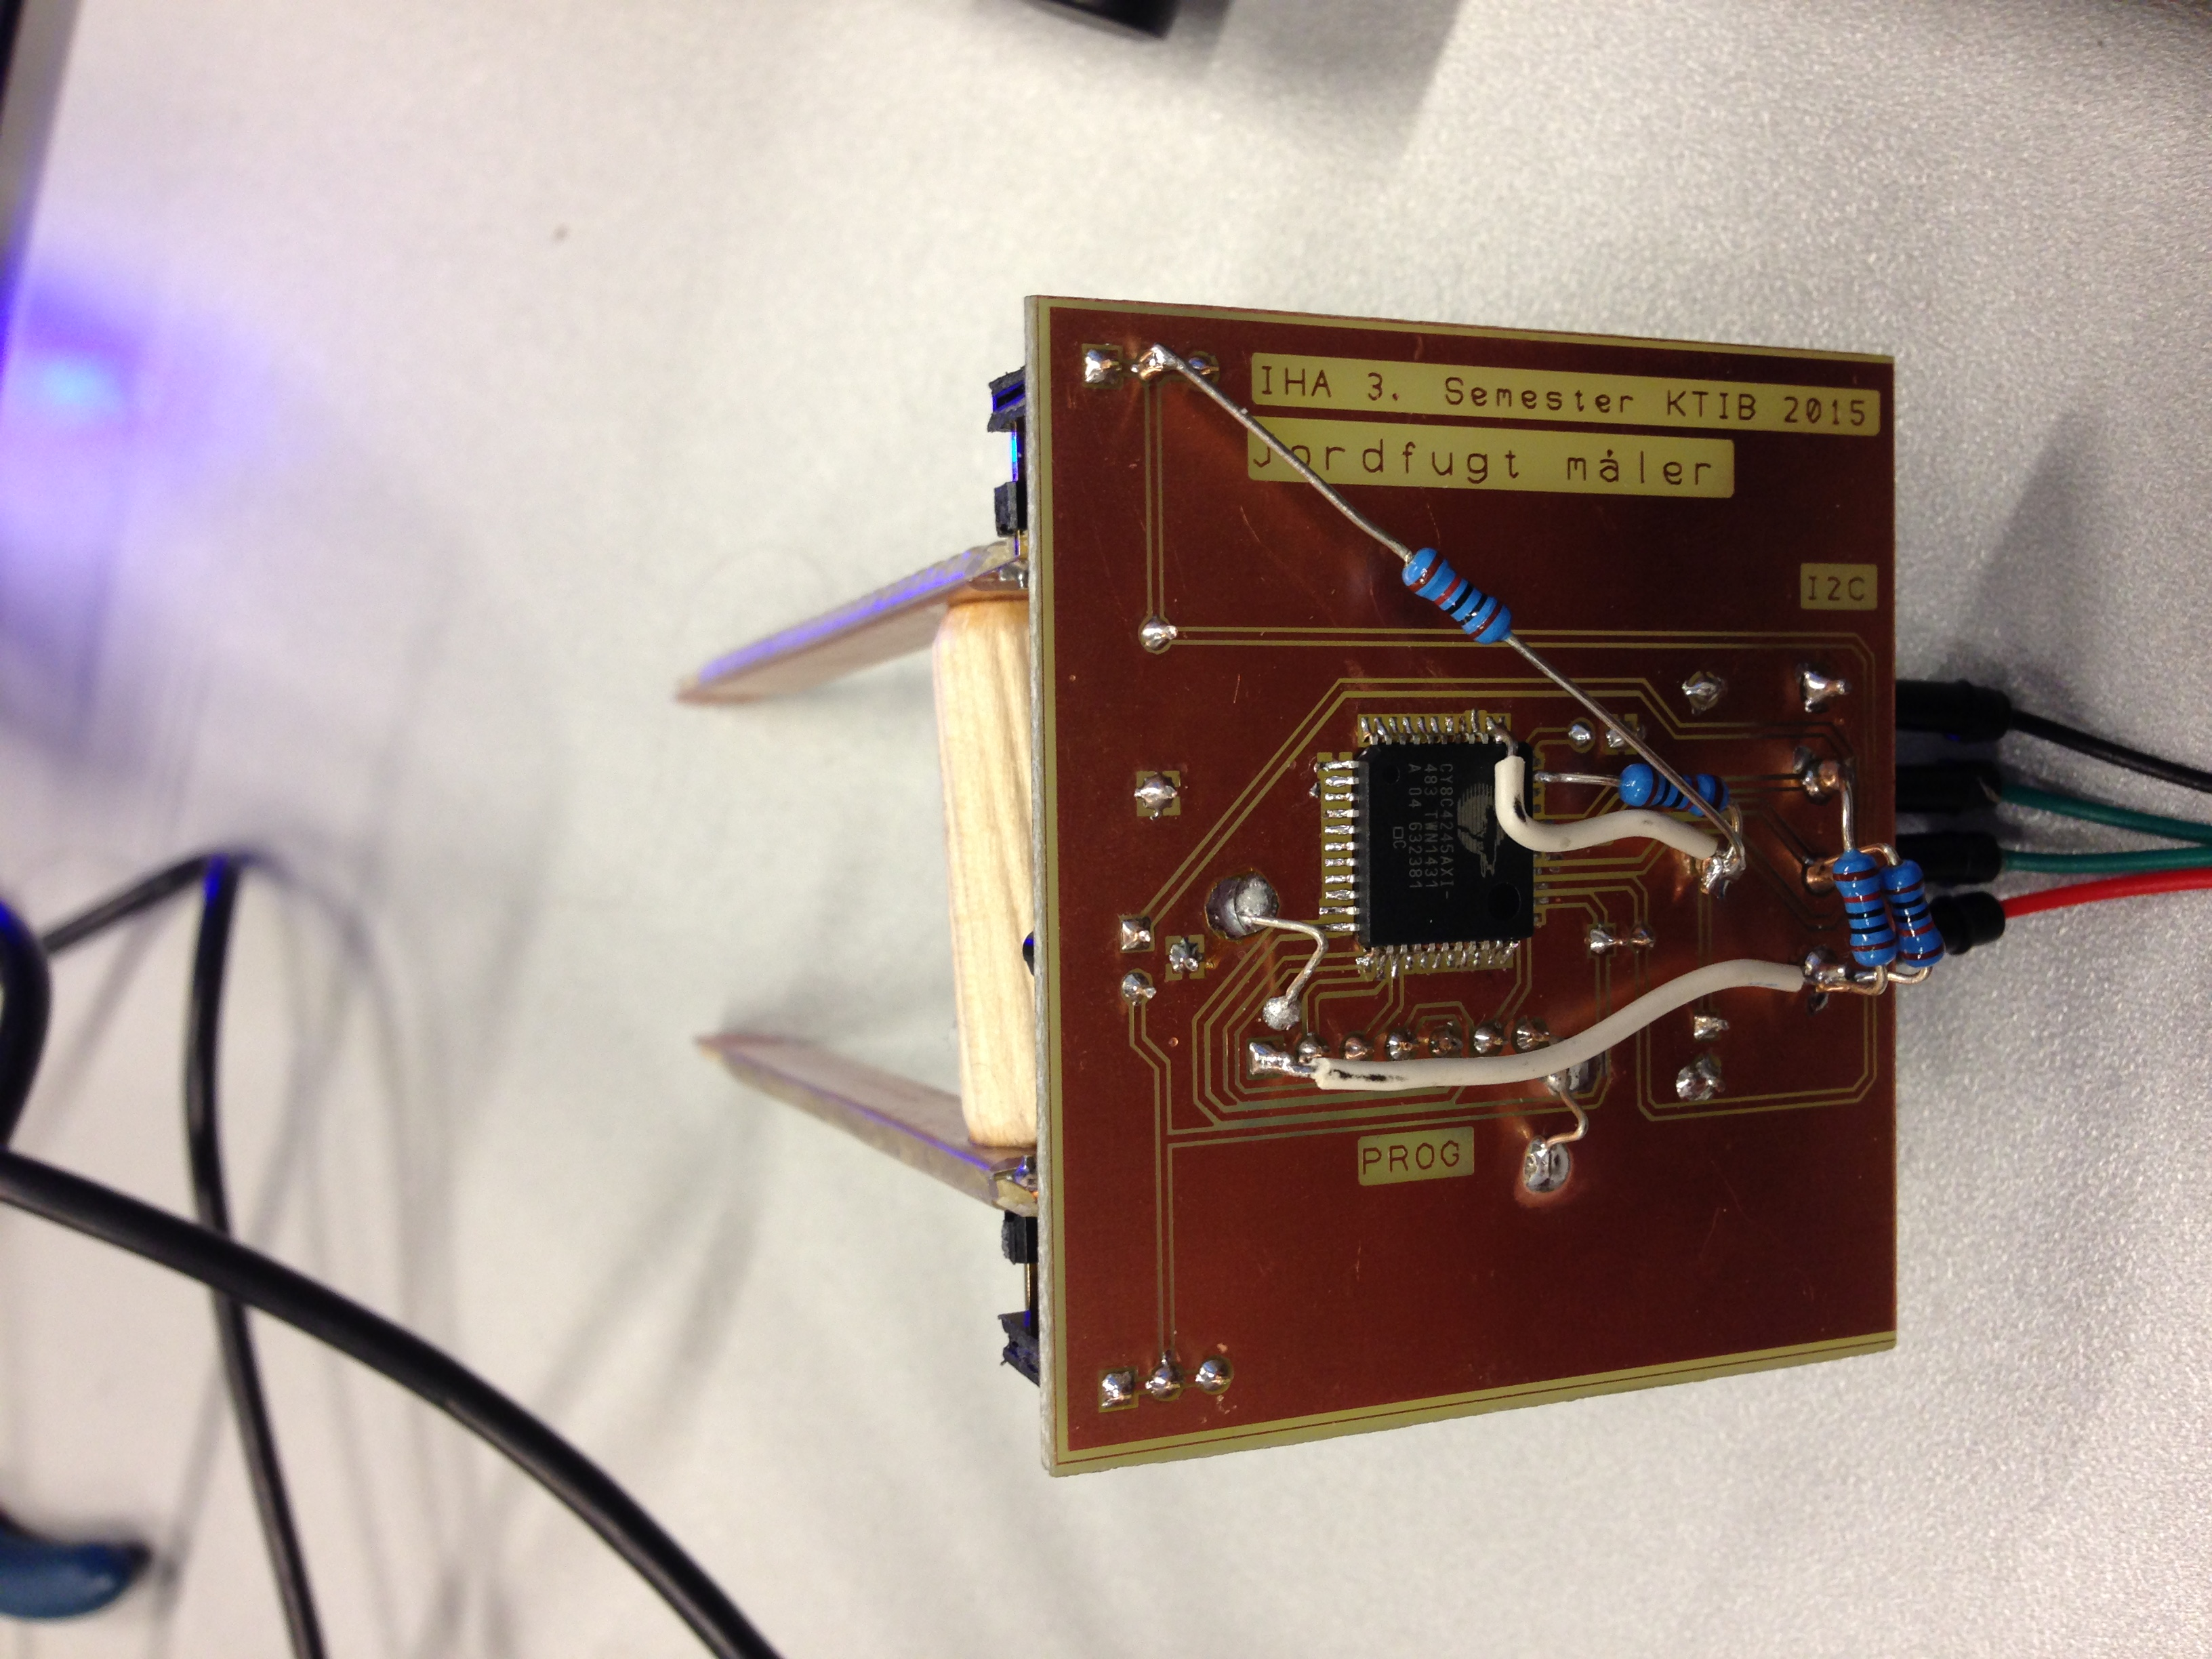
\includegraphics[scale=0.1]{HardwareArkitektur/Sensore/Jordfugt_billeder/Print_2.jpg}
	\caption{Printplade set fra bunden}
	\label{photo:Print_2}
\end{figure} 

Det ses på fig.\ref{photo:Print_2} at der er foretaget nogle modifikationer ved printet. Dette skyldes, at der i første iteration var glemt at implementere pull-up modstande, samt at DesignSpark, fejlagtigt havde valgt at ligge stel sammen med forsyningen. 
Diagrammet blev derfor i 2.iteration modificeret til følgende fig.\ref{photo:Diagram_jordfugt}.

\begin{figure}[H]
	\centering 
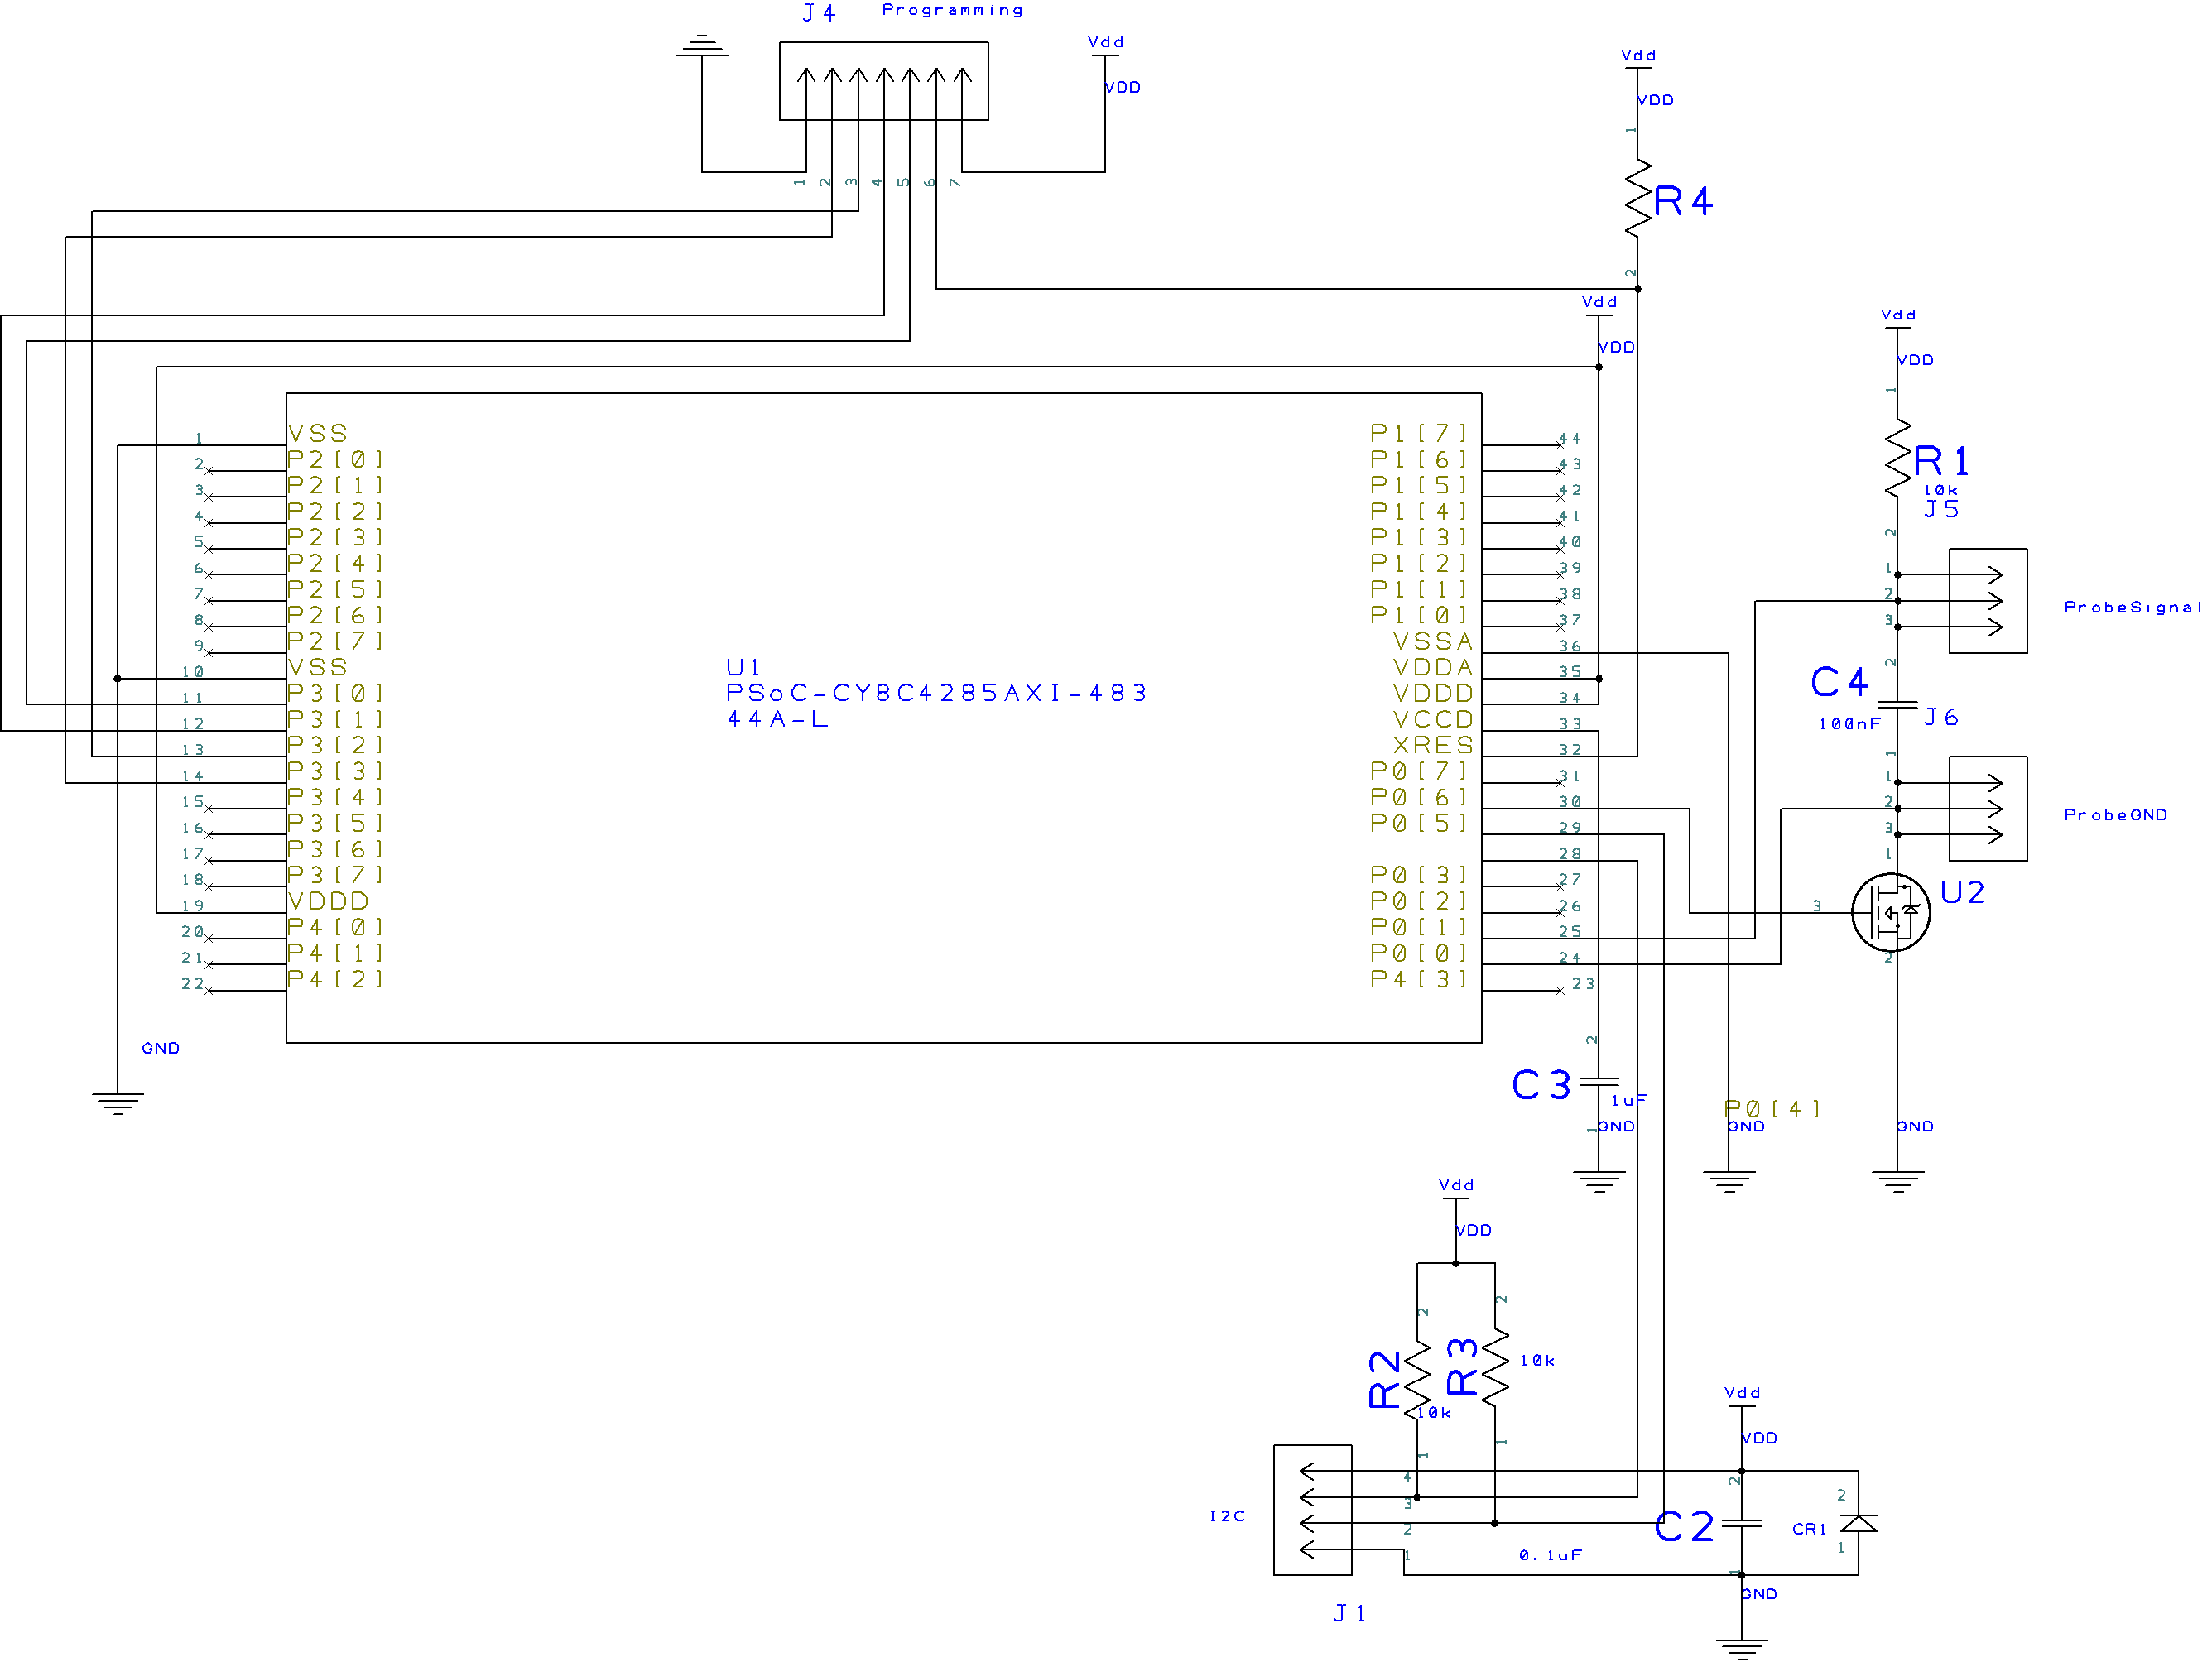
\includegraphics[scale=0.2]{HardwareArkitektur/Sensore/Jordfugt_billeder/Diagram_jordfugt.png}
	\caption{Diagram over jordfugtsensoren}
	\label{photo:Diagram_jordfugt}
\end{figure} 

Det ses af diagrammet på fig.\ref{photo:Diagram_jordfugt} at der er trukket pins ud til at programmere PSoC'en. Ved at forbinde disse til Pioneer-kittet kan PSoC'en programmeres igennem en PSoC-5, og på denne måde undgå at skulle købe en ekstern programmeringsenhed. Det viste sig dog at der var flere problemer da det nye print blev lavet. Der kunne sagens kommunikeres med PSoC'en igennem programmerings-pins'ne. Men derimod var det umuligt at få nogen funktionalitet ud af den. Der blev brugt dage på at finde en løsning på problem med desværre uden resultat. Det blev derfor besluttet at lave et shield til pioneer-kittet.

\begin{figure}[H]
	\centering 
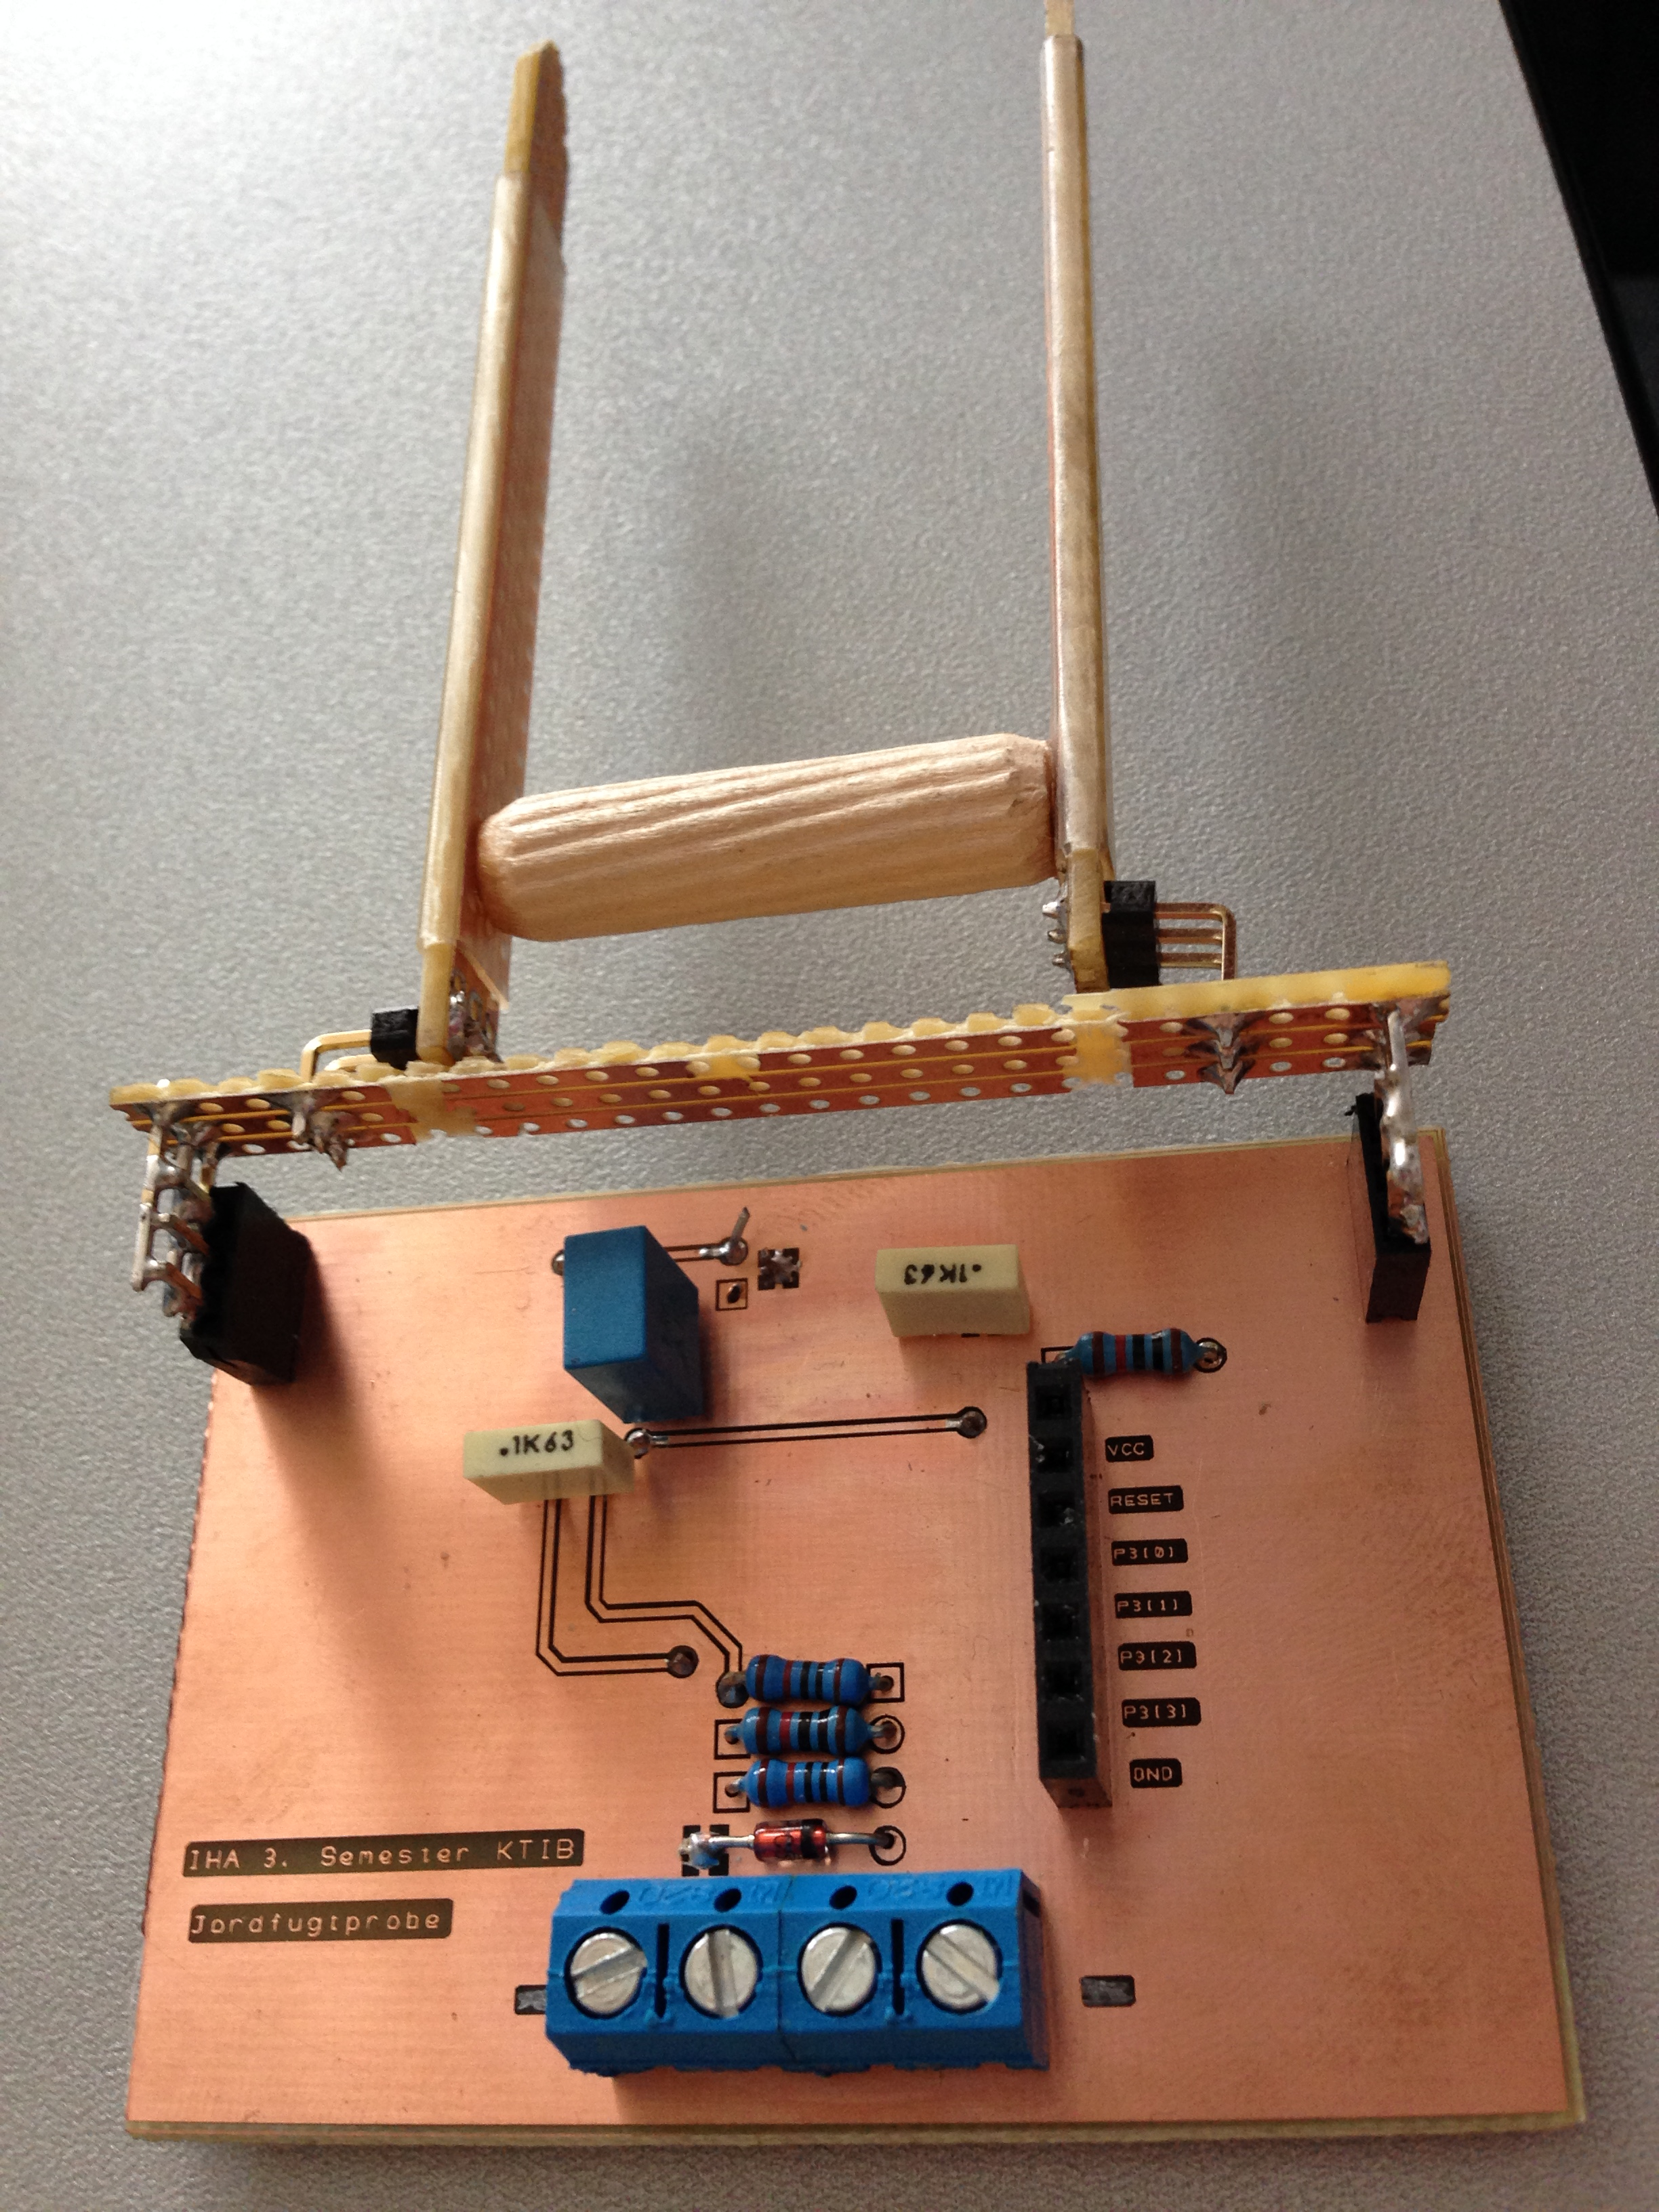
\includegraphics[scale=0.08]{HardwareArkitektur/Sensore/Jordfugt_billeder/print_ny_top.JPG}
	\caption{Det nye print set fra oven}
	\label{photo:print_ny_top}
\end{figure} 

\begin{figure}[H]
	\centering 
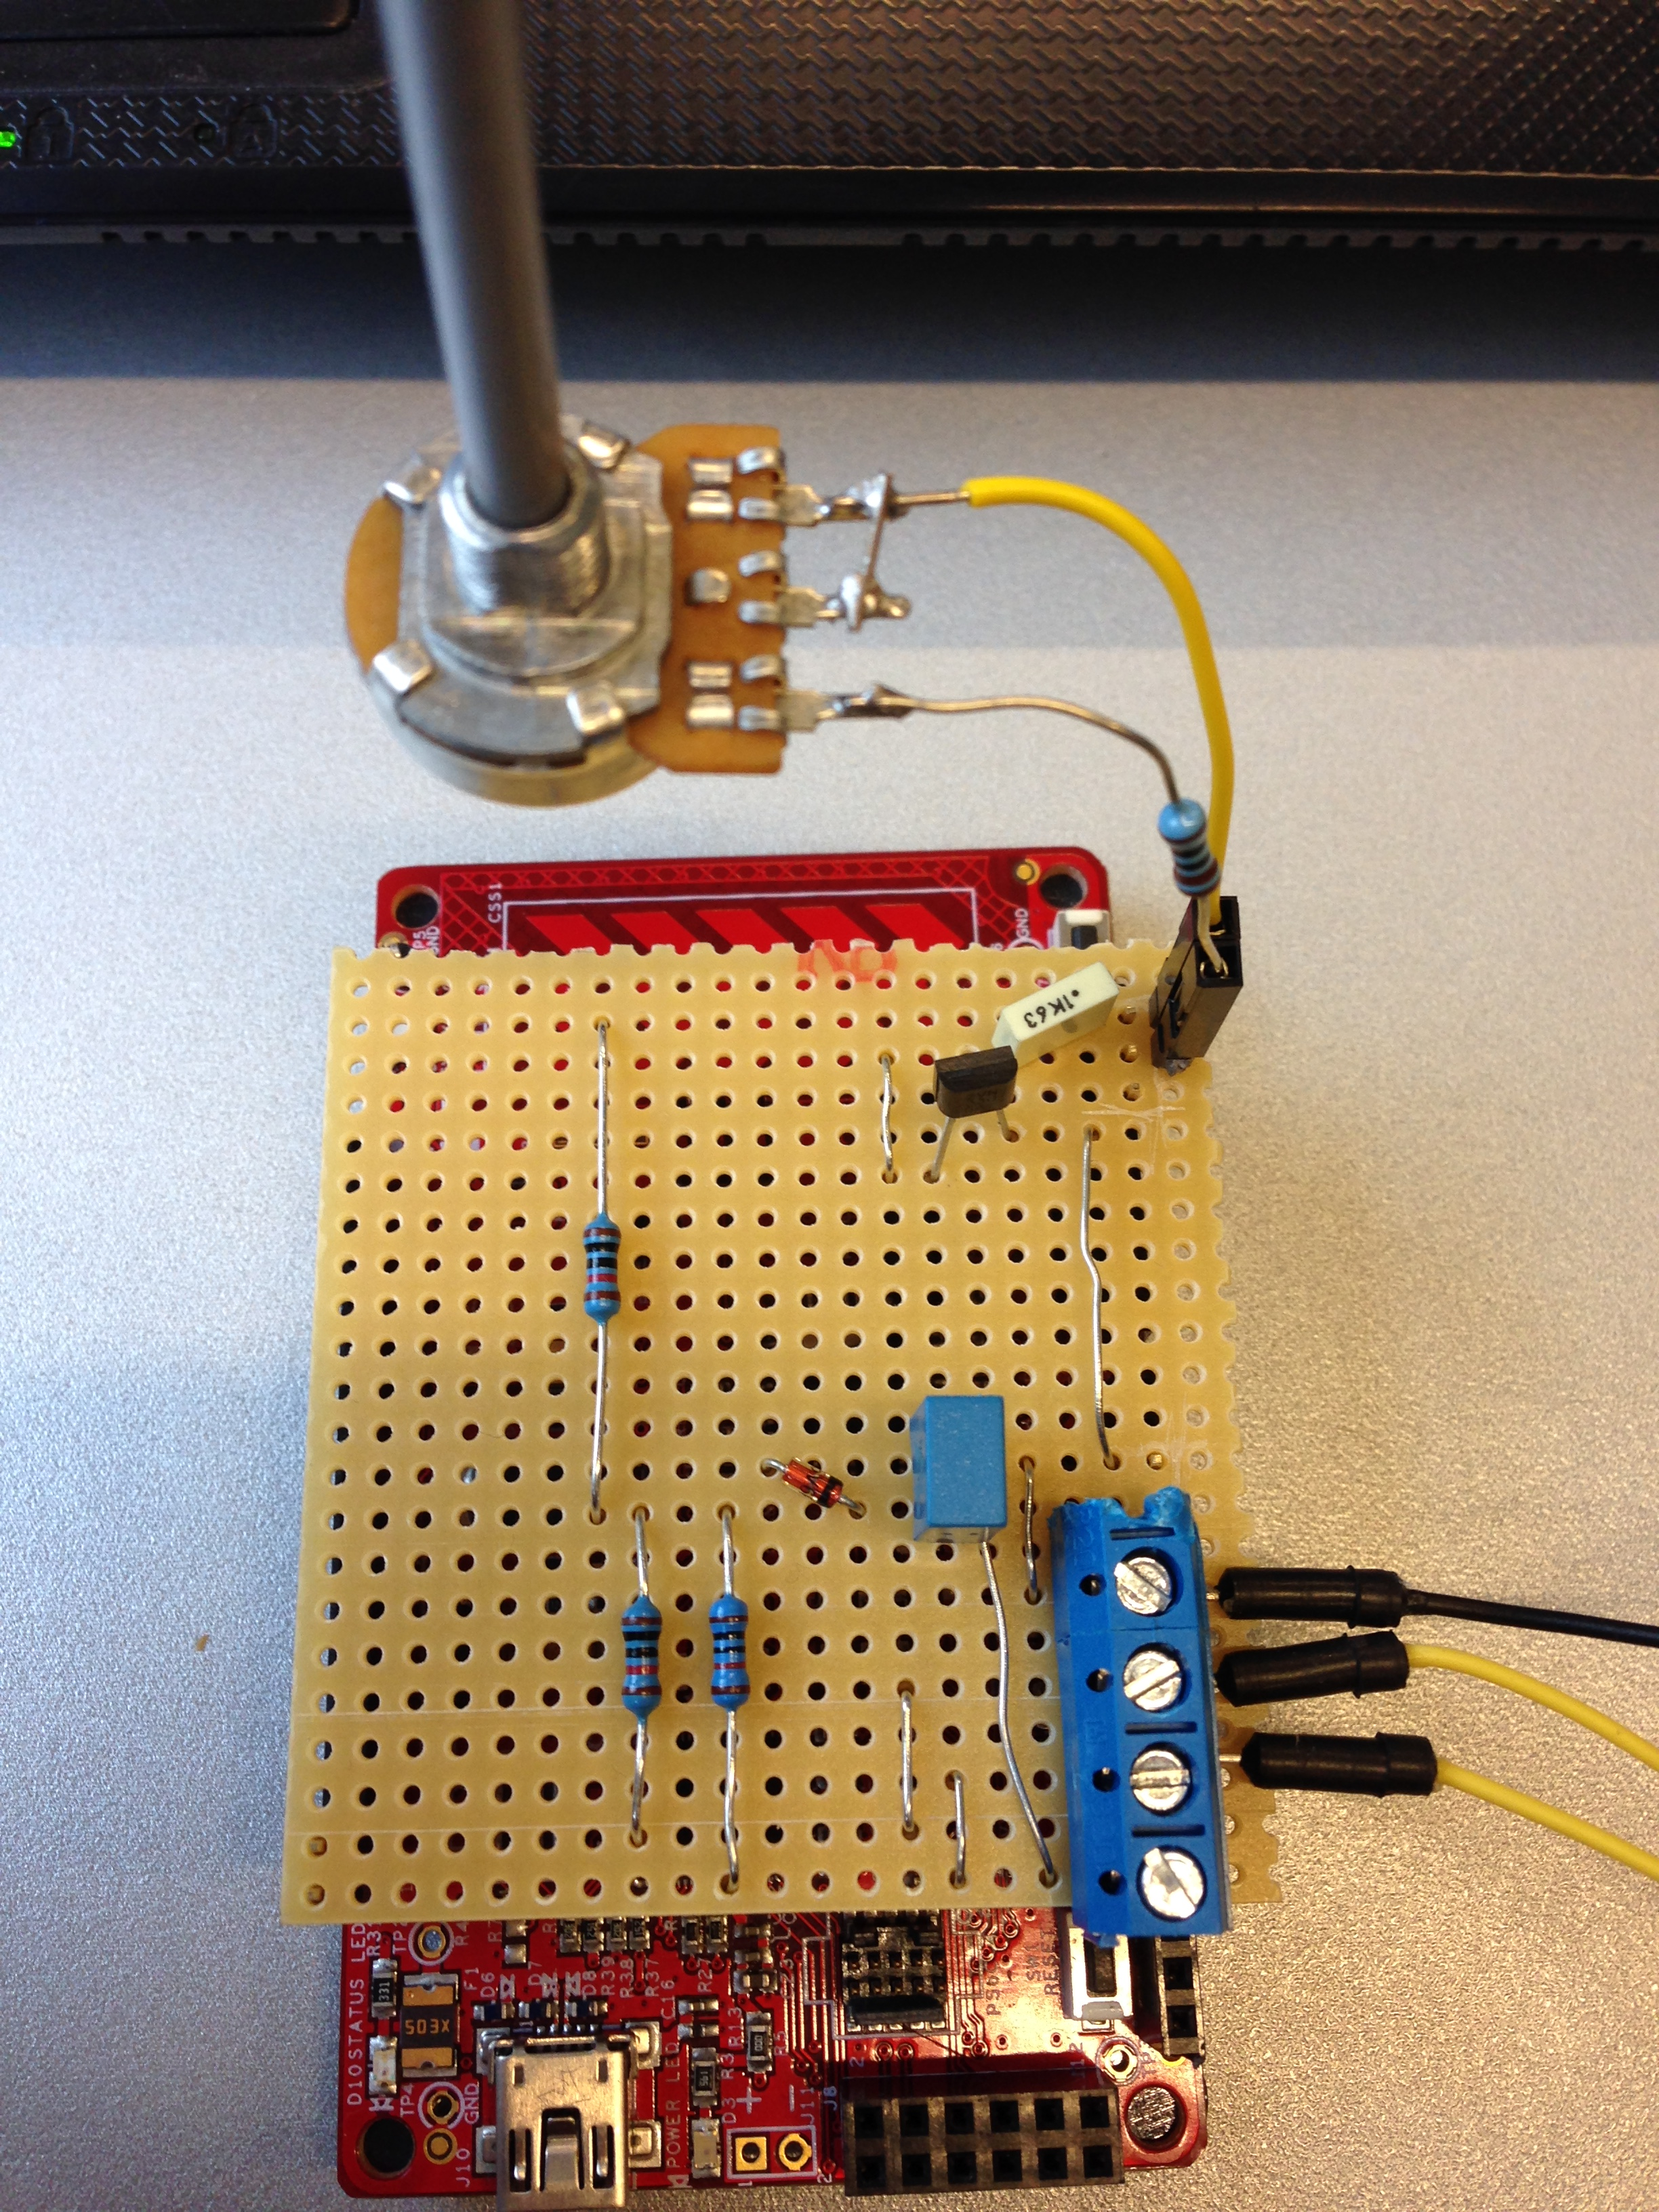
\includegraphics[scale=0.08]{HardwareArkitektur/Sensore/Jordfugt_billeder/shield.JPG}
	\caption{Shield. Potientiometeret emulerer proben}
	\label{photo:shield}
\end{figure} 

\subsubsection{Præcision og afvigelse}
Der blev kørt et testprogram med det nye shield på måling i jord. Da hverken ledeevnen eller fugtigheden i jorden er kendt, måltes først jorden da den var tør. Her måltes fugtigheden til 3,5\%. Efterfølgende tilsattes 10\% vand og brugte denne blanding til at udregnede afvigelsen. Afvigelsen blev beregnet til 1,58\% med 95\% konfidens. 

\begin{figure}[H]
	\centering 
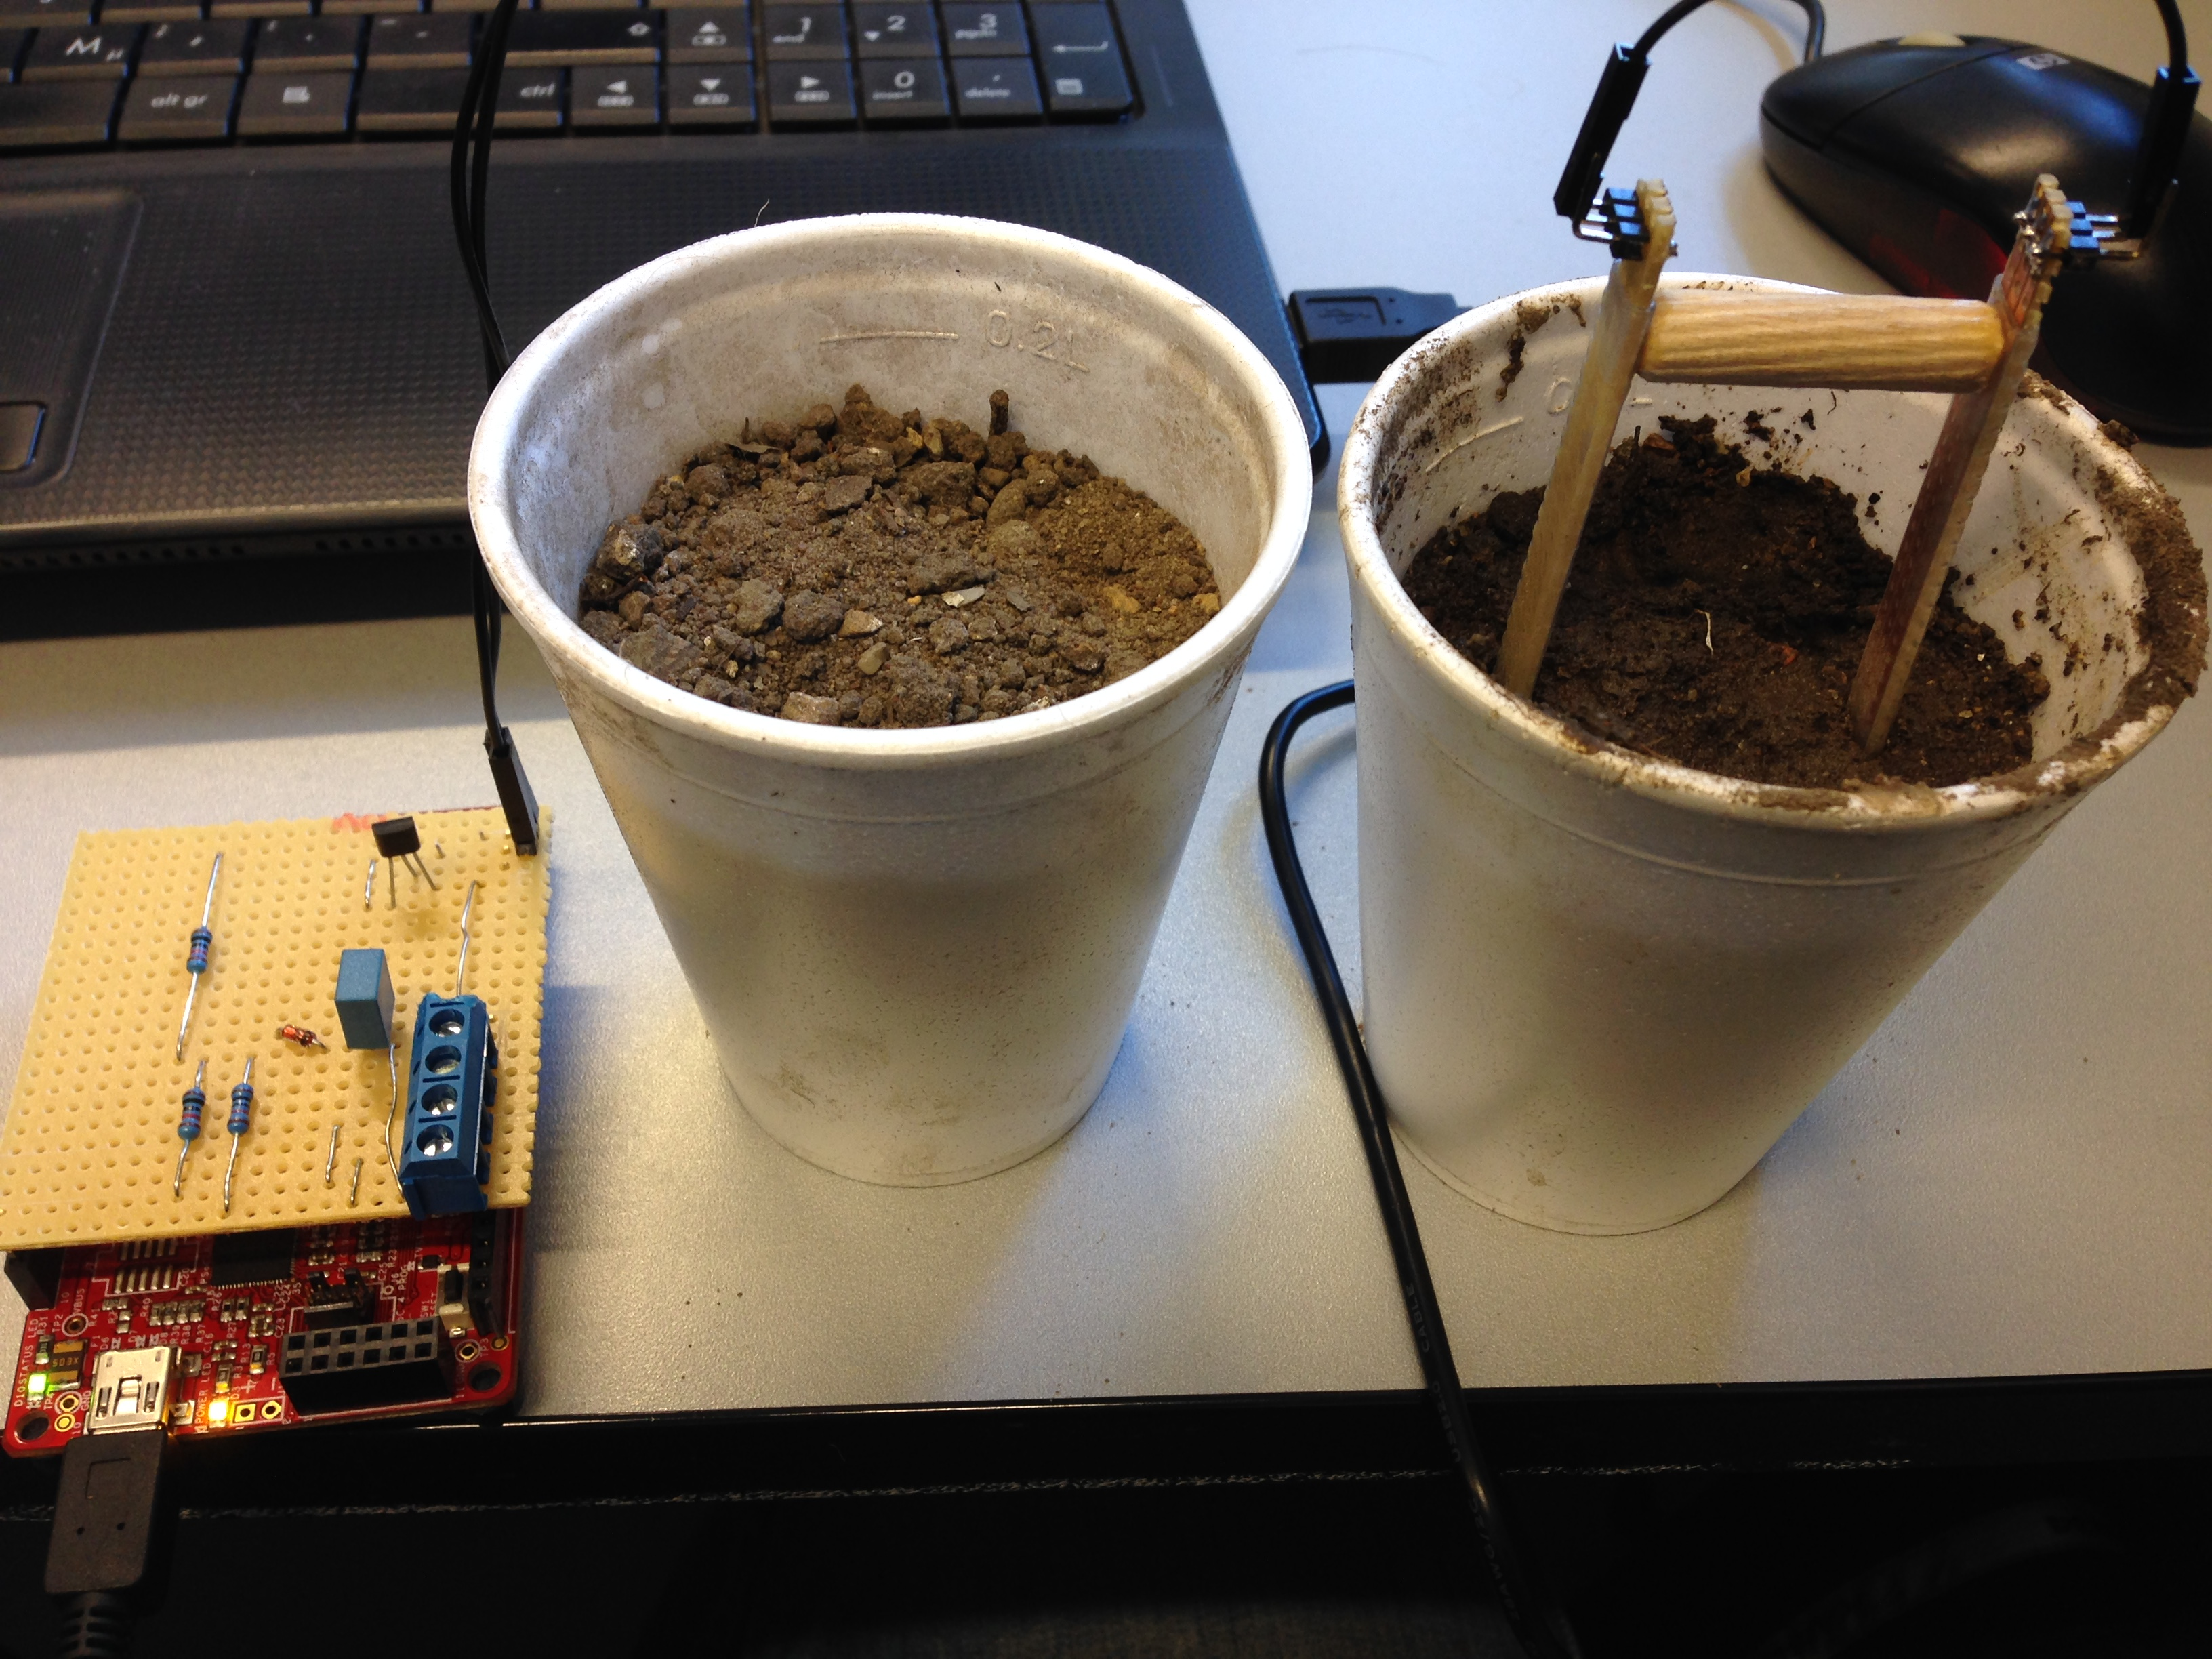
\includegraphics[scale=0.08]{HardwareArkitektur/Sensore/Jordfugt_billeder/test_maling.JPG}
	\caption{Test måling}
	\label{photo:shield}
\end{figure} 

\begin{figure}[H]
	\centering 
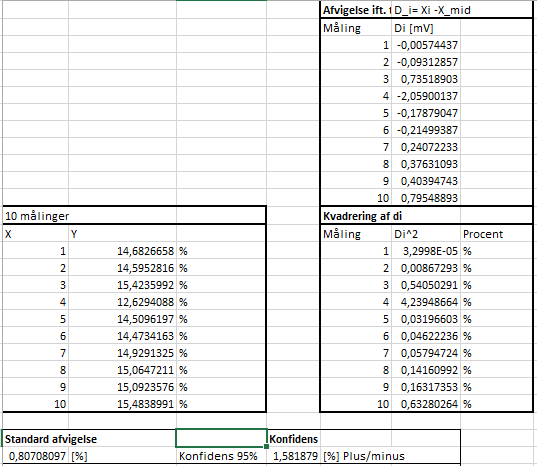
\includegraphics[scale=1]{HardwareArkitektur/Sensore/Jordfugt_billeder/afvigelse.PNG}
	\caption{Udregning af afvigelsen}
	\label{photo:shield}
\end{figure} 

Selve præcisionen af proben er 12 bit og 5V. Dette giver en opløsning på 1.2mV. Omregnet til opløsning af procentenheden bliver det 0.061.